% Modelo de Dissertação do Mestrado em Informática da PUC - Alterado para cumprir a normalização de 2011
%\documentclass[a4paper,brazil,ruledheader,normaltoc,capchap]{abnt}

% Para impressão frente e verso (normalização 2011)
\documentclass[a4paper,brazil,ruledheader,normaltoc,capchap,twoside,openany]{abnt_pucmg_utf8}

% Não esquecer das alterações no arquivo abnt.cls
% Se estiver usando o Kile no Ubuntu o arquivo fica armazenado em /usr/share/texmf/tex/latex/abntex.
% Comentar a linha 967 
% \vspace*{30pt}% - Linha comentada para reduzir o espaçamento entre o topo da página e o título \chapter
% Alterar a linha 1143
% \vspace*{-30pt} % - Parâmetro alterado de 30pt para -30pt para reduzir o espaçamento entre o top da página e o título do apêndice
% Alterar a linha 985
%\vspace*{-30pt}\par % - Parâmetro alterado de 0pt para -30pt para reduzir o espaçamento entre o top da página e o título \chapter*
% Alterar a linha 991
% Parâmetro alterado de 45pt para 30pt para reduzir o espaçamento entre o texto e o título \chapter*

% Não esquecer das alterações no arquivo acronym.sty
% Se estiver usando o Kile no Ubuntu o arquivo fica armazenado em /usr/share/texmf-texlive/tex/latex/acronym
% Alterar a linha 225
%\item[\protect\AC@hypertarget{#1}{\acsfont{\normalfont{#2}}} --] #3% - Inserir separador entre acrônimo/descrição e remover o negrito com o normalfont

% Pacote para definir explicitamente as margens das páginas
\usepackage[a4paper,left=3cm,right=2cm,top=3cm,bottom=2cm]{geometry}

%\usepackage{units}
% Utilize da seguinte forma \unit[78,6]{mA}

% Pacote para gerenciar siglas
\usepackage[printonlyused]{acronym}

% Merge em duas células (linhas diferentes)
\usepackage{multirow}

% Pacote para citação e referências seguindo ABNT no sistema (AUTOR, Data)
%\usepackage[alf, bibjustif,abnt-emphasize=bf]{abntcite}
\usepackage[alf, abnt-emphasize=em, abnt-thesis-year=title]{abntcite}
% @article An article from a journal or magazine 
% @inproceedings An article in a conference proceedings
% Força que o tipo de ênfase no nome do simpósio seja em caixa alta
\renewcommand{\emph}{\textsc}

% Pacote para múltiplos arquivos .bib
\usepackage{multibib}
%\newcites{pub}{Refer\^encias das publica\c{c}\~oes}

% Pacote de adequação do formato ABNT para normas da PUCMinas
\usepackage{abnt-PPGInf-PUCMG}

% Pacotes utilitários
\usepackage{graphicx}
\usepackage{longtable}

% Pacote para fixar a figura no local desejado
\usepackage{float}

% Pacote para adicionar simbolos as informações de rodapé
\usepackage[symbol]{footmisc}

\usepackage[all]{xy}
%\usepackage[tight]{subfigure}	% Permite a criação de subfiguras
\usepackage{url,amsmath}	% Permite melhorias na codificação de fórmulas
%\usepackage{amsthm}		% Permite melhorias na escrita de teoremas
\usepackage{amssymb}		% Permite utlização de simbolos matemáticos avançados


% Alterar o espaçamento da margem no algoritmo

\newcommand{\source}[1]{\caption*{Source: {#1}} }

\usepackage{setspace}

% Pacote para rotação de tabelas/figuras
\usepackage{rotating}

% Pacotes para criação de cronograma/tabela colorida
\usepackage{color}
\usepackage{array}
\usepackage{longtable}
\usepackage{colortbl}

%\definecolor{lightgray}{gray}{0.9}

% Pacote para possibilitar o uso do setboolean para forçar formatos de página diferentes do padrão do documento
\usepackage{ifthen}

% Para inserir captions (nova normalização 2011)
\usepackage[size=normalsize,labelfont=bf,textfont={bf},labelsep=endash]{caption}
\captionsetup[subfloat]{labelfont=bf,textfont={bf}}

% Usado para reduzir espaçamentos entre itens (alíneas, enumerações) com o compactitem
\usepackage{paralist}

% Alterar para sequencial a numeração de figuras e tabelas
\captionsetup{figurewithin=none}
\captionsetup{tablewithin=none}

\setlength{\LTcapwidth}{\textwidth}

% Para o subsubsection aparecer no sumário 
\setcounter{tocdepth}{3}
\setcounter{secnumdepth}{3}

% Para inserir referências via links - não funciona para abntex
%\usepackage[colorlinks=true,pdfstartview=FitV,linkcolor=blue,citecolor=blue,urlcolor=blue,hyperindex,pagebackref=true,pdftex,breaklinks]{hyperref}
%\usepackage[pdftex]{hyperref}

% Para criar lista de gráficos
\floatstyle{plaintop}
\newfloat{grafico}{H}{loq}
\restylefloat*{grafico}
\floatname{grafico}{Gráfico} 

% Para gerar subfiguras usando o subfloat
\usepackage{subfig}
\usepackage{caption}
\usepackage{subcaption}
%\newsubfloat[position=bottom,listofformat=subsimple]{grafico}

\usepackage{listings}
\usepackage{color}
\definecolor{dkgreen}{rgb}{0,0.6,0}
\definecolor{gray}{rgb}{0.5,0.5,0.5}
\definecolor{mauve}{rgb}{0.58,0,0.82}
\definecolor{gray}{rgb}{0.4,0.4,0.4}
\definecolor{darkblue}{rgb}{0.0,0.0,0.6}
\definecolor{lightblue}{rgb}{0.0,0.0,0.9}
\definecolor{cyan}{rgb}{0.0,0.6,0.6}
\definecolor{darkred}{rgb}{0.6,0.0,0.0}


\usepackage[margin=2.5cm]{geometry}
\usepackage{tabularx}


\lstset{
  basicstyle=\ttfamily\footnotesize,
  columns=fullflexible,
  showstringspaces=false,
  numbers=left,                   % where to put the line-numbers
  numberstyle=\tiny\color{gray},  % the style that is used for the line-numbers
  stepnumber=1,
  numbersep=5pt,                  % how far the line-numbers are from the code
  backgroundcolor=\color{white},      % choose the background color. You must add \usepackage{color}
  showspaces=false,               % show spaces adding particular underscores
  showstringspaces=false,         % underline spaces within strings
  showtabs=false,                 % show tabs within strings adding particular underscores
  frame=none,                   % adds a frame around the code
  rulecolor=\color{black},        % if not set, the frame-color may be changed on line-breaks within not-black text (e.g. commens (green here))
  tabsize=2,                      % sets default tabsize to 2 spaces
  captionpos=b,                   % sets the caption-position to bottom
  breaklines=true,                % sets automatic line breaking
  breakatwhitespace=false,        % sets if automatic breaks should only happen at whitespace
  title=\lstname,                   % show the filename of files included with \lstinputlisting;
                                  % also try caption instead of title  
  commentstyle=\color{gray}\upshape
}


\lstdefinelanguage{XML}
{
  morestring=[s][\color{mauve}]{"}{"},
  morestring=[s][\color{black}]{>}{<},
  morecomment=[s]{<?}{?>},
  morecomment=[s][\color{dkgreen}]{<!--}{-->},
  stringstyle=\color{black},
  identifierstyle=\color{lightblue},
  keywordstyle=\color{red},
  morekeywords={xmlns,xsi,noNamespaceSchemaLocation,type,id,x,y,source,target,version,tool,transRef,roleRef,objective,eventually}% list your attributes here
}

\usepackage{algpseudocode}
\usepackage{algorithm}
\usepackage[inline]{enumitem}
% define estilo de posicionamento na caixa
\newsavebox{\leftfig}
\newsavebox{\rightfig}

%\renewcommand{\ALG@name}{Algoritmo}
%\renewcommand{\listalgorithmname}{Lista de Algoritmos}


\citeoption{abnt-etal-cite=1, abnt-and-type=e}

% the bibtex style generates this command, but it's not defined
%\newcommand{\optionaltextstyle}{}


\newcommand{\optionaltextstyle}{}

% PRÉ-TEXTUAIS %%
\begin{document}

% Para forçar que elementos pré-textuais (da capa até o sumário) sejam impressos no anverso da folha
\setboolean{@twoside}{false}

\autor{Pedro Pongelupe Lopes}

% Coloque o título em caixa alta. É o padrão da PUC.
% Vá no arquivo abnt-PPGInf-PUCMG.sty e procure por esse título (linha 575). Altere para o seu título em caixa alta. Isso será utilizado na folha de aprovação.
\titulo{
PONDIÔNSTRACKER: A FRAMEWORK BASED ON GTFS-RT TO IDENTIFY DELAYS AND ESTIMATE ARRIVALS DYNAMICALLY IN PUBLIC TRANSPORTATION NETWORK}


\orientador[Advisor:]{Prof. Humberto T.
\\ Marques-Neto}

% Se não tiver, co-orientador, comente a próxima linha.
%\coorientador[Co-orientador:]{Professor}

% Texto
\comentario{Dissertation presented to the Graduate
Program in Informatics at Pontifical Catholic
University of Minas Gerais, as a partial requirement to obtain Master’s degree in Informatics.
}


% Instituição


% Local
\local{Belo Horizonte}

% Data
\data{2023}
\capa
%Para forçar que a ficha catalográfica seja impressa no verso da folha de aprovação
\setboolean{@twoside}{false}

% Gera a folha de rosto
\folhaderosto

% Ficha catalográfica
% Ficha catalográfica
% INCLUIR O ARQUIVO PDF GERADO PELA BIBLIOTECA COMO FIGURA.
\begin{figure}[h!]
	\vspace*{-3.3cm}
	\hspace*{-3cm}
%	% Suponha o nome do arquivo em pre-texto/ficha-catalografica/fichacatalografica.pdf
	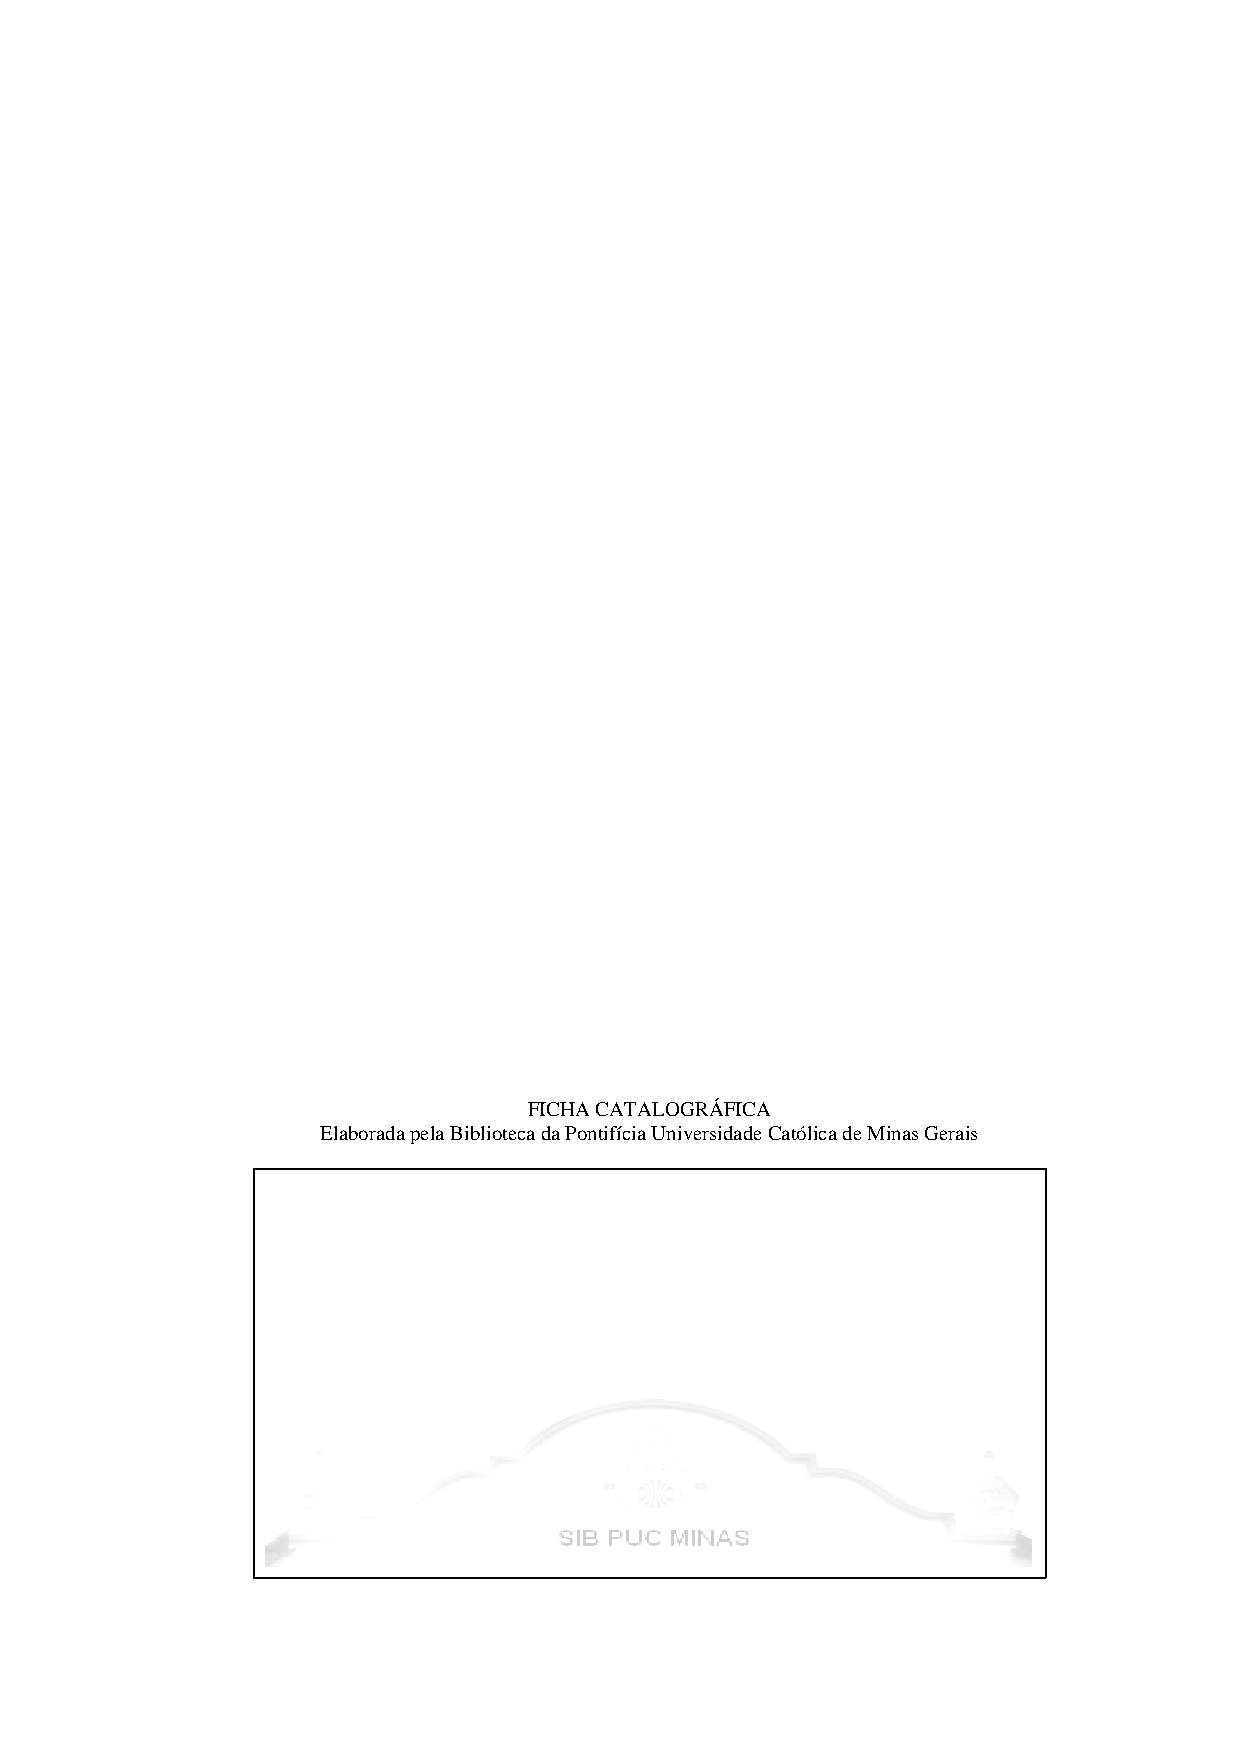
\includegraphics{pre-texto/ficha-catalografica} 
	\newpage
\end{figure}

% Para forçar que elementos pré-textuais (da capa até o sumário) sejam impressos no anverso da folha
\setboolean{@twoside}{false}

% Folha de aprovação
% Termo de Aprovação

% Texto da aprovação
\textoaprovacao{Dissertation presented to the Graduate Program in Informatics as a
partial requirement for qualification to
the Master degree in Informatics from
the Pontifical Catholic University of Minas Gerais}

% Primeira assinatura
\primeiroassina{Prof. Dr. Humberto Torres Marques-Neto -- PUC Minas (Advisor)}

% Segunda assinatura
\segundoassina{Prof. Dr. Silvio Jamil Ferzoli Guimarães -- PUC Minas (Examining Board)}

% Terceira assinatura
\terceiroassina{Prof. Dr. Davide Bacciu --  \\Università di Pisa (Examining Board)}

% Quarta assinatura
%\quartoassina{}

% Data da defesa
\localdia{Belo Horizonte, December 04, 2023.}

% Gera o termo de aprovação
\termodeaprovacao	


% Dedicatória
%% Dedicatória
%\newpage

% Espaçamento do topo da página até o texto da dedicatória
%\vspace*{22cm}

% Espaçamento na esqueda
%\hspace{8cm}\begin{minipage}{.60\textwidth}
            %\textit{texto de dedicatoria}
            %\end{minipage}

% Agradecimentos
% Agradecimentos
\chapter*{Agradecimentos}
\begin{center}
	\normalsize
	A conclusão dessa dissertação simboliza um vitória pessoal gigantesca. E não seria possível sem uma série de pessoas envolvidas. 
 
    Em especial, à minha namorada Naraiane que, neste ano de 2023, vem compartilhando comigo as mais variadas experiências: alegrias, tristezas, incertezas e boas risadas. Muito obrigado por ter me levado ao hospital naquele dia, sou eternamente grato.
    Sem o seu companheirismo diário e conversas importantíssimas que tivemos enquanto preparávamos uma boa receita degustando um bom vinho, essa dissertação não existiria.

    Ao Professor Humberto que me acompanha em mais uma etapa da minha trajetória acadêmica, certamente a mais complexa para mim, até então. Obrigado por embarcar nas ideias mirabolante que tenho, sempre me inspirando a ser um pesquisador melhor.

    À minha família que sempre me apoiou e me proporcionou alento em momentos difíceis, especialmente aos meus pais, Soraya e Eustáquio. Também agradeço à Elaine e Toninho que sempre me tiveram por perto e me mostram mais sobre o mundo. Obrigado
    por terem me acolhido em Ouro Branco.

    Aos meus amigos por vivenciar o processo todo comigo, especialmente durante a pandemia que factualmente moramos juntos. Eram ótimas risadas e comes e bebes de qualidade duvidosa. Ao Daniel, Banana, obrigado em dobro por me acompanhar em fazer o mestrado, me incentivou muito em iniciar, continuar e finalizar, e também obrigado, pela comemoração de aniversário na carreta furacão. Não poderia deixar de salientar como o excelentíssimo Patrick Galdino me diverte em inúmeras ocasiões e faz um ótimo feijão tropeiro. Também ao 
    Paulinho que além de cupido, é um ótimo colega de trabalho e amigo. Toto, João, Vic, Alaor e outros, muito obrigado pela amizade sincera.

    Finalmente, agradeço ao Jorge Ben Jor, FBC e Don L que estiveram preenchendo o ambiente com ótimas ideias 
    enquanto essa dissertação foi escrita. Inclusive, estou escutando Jorge Ben enquanto termino este agradecimento. Salve Jorge! Viva São Jorge!

    Venceremos!
	
\end{center}

 

% Epígrafe
% Epígrafe
\newpage

% Espaçamento entre topo da página e texto da epígrafe
\vspace*{10cm}
% Espaçamento na esqueda
\hspace{4cm}\begin{minipage}{.51\textwidth}

% Texto da epígrafe
\textit{``Hay que endurecerse, pero sin perder \\la ternura jamás.'' }

%Nome do autor
\begin{flushright}\itshape Ernesto 'Che' Guevara
\upshape\end{flushright}

\end{minipage}

% Abstract
% Abstract
\begin{abstract}
% Diminuir espaçamento entre título e texto
\vspace{-1cm}
% Texto do resumo, em inglês: sem paragrafo, justificado, com espaçamento 1,5 cm
\onehalfspacing
\noindent

A smart city Public Transportation Network provides mobility services to millions of people daily. 
Urban computing provides a
toolkit to handle acquisition, integration, and analysis, which translates to the improvement of the human mobility
of the citizens, mitigating and notifying delays, for instance.
Regarding the PTN, many methods rely on two specifications: \textit{General Transit Feed Specification} (GTFS) and \textit{General Transit Feed Specification Real-Time} (GTFS-RT). The first represents the static schedule information, and the second introduces real-time updates from trips, services, and vehicle positions. Despite the qualitative leap with the GTFS-RT specification, GTFS-RT
is not as well-adopted as the GTFS because of the non-existence of a matching identifier between the static and real-time data. In this context, we present \textit{PondiônsTracker}\footnote{Available at \url{https://github.com/Pongelupe/PondionsTracker/}} which is a {\em loose coupling} Java framework designed for enriching GTFS data with real-time data to enable delays analysis and to estimate arrivals. So, we present \textit{PondiônsTracker-BH}\footnote{Available at \url{https://github.com/Pongelupe/PondionsTracker-BH}} that is a \textit{PondiônsTracker}'s specialization created to
deal with Belo Horizonte's PTN particularities originating from Belo Horizonte's real-time \ac{API} 
which we collected every minute for eleven days straight in July and August 2023, summarizing over 246 million entries 
representing almost 30 Gigabytes.
\textit{PondiônsTracker-BH} presented a $76.08\%$ of the matched trips for the schedule during the observation period, 
then $156,628$ out of $205,884$ scheduled trips were identified in the real-time data. Analyzing these $156,628$ matched trips,
we show the delays focus and show that the delays in Belo Horizonte are spatial and temporal related
and are {\em log-normal} distributed. In other words, most of the delays in Belo Horizonte occur at a few bus stops, and these stops are \textit{physically} close to each other and share the same \textit{temporal} patterns.

% Espaçamento para as palavras-chave
\vspace*{.75cm}

% Palavras-chave: sem parágrafo, alinhado à esquerda
\noindent Keywords: Urban Computing, Human Mobility, Complex Networks, Public Transportation Network.
% Segunda linha de palavras-chave, com espaçamento.
%\indent\hspace{1.4cm} Keyword.

\end{abstract}


% Resumo
% Resumo
\begin{resumo}
% Diminuir espaçamento entre título e texto
\vspace{-1cm}

% Texto do resumo: sem paragrafo, justificado, com espaçamento 1,5 cm
\onehalfspacing

\noindent 
  O ano de 2020 vem sendo marcado pelo espalhamento em níveis globais de uma nova doença
  infecciosa, a COVID-19. Técnicas de computação urbana vem sendo empregadas para amenizar
  os danos sociais gerados pela pandemia, como utilização de rastreio de contato
  para medidas de isolamento social menos abruptas. Este projeto explorará evidências relacionadas aos 
  boletins epidemiológicos e dados de mobilidade para analisar a transmissão e disseminação
  da COVID-19 e propor medidas que minimizem os impactos da doença na sociedade. As análises
  buscam suavizar as medidas de isolamento social e planejamento do transporte urbano na cidade,
  assim propondo um método de rastreio de contatos.

% Espaçamento para as palavras-chave
\vspace*{.75cm}

% Palavras-chave: sem parágrafo, alinhado à esquerda
\noindent Palavras-chave: Computação Urbana, Mobilidade, Saúde, Redes Complexas
% Segunda linha de palavras-chave, com espaçamento.
%\indent\hspace{2cm}Palavra.

\end{resumo}

\makeatletter
\renewcommand\numberline[1]{
	\leftskip 0em
	\rightskip 1.6em
	\parfillskip -\rightskip
	\parindent 0em
	\@tempdima 2.0em
	\vspace{0em} \advance\leftskip \@tempdima \null\nobreak\hskip -\leftskip
	FIGURE \normalfont #1 -- }
\makeatother

% Lista de figuras
\listoffigures

\makeatletter
\renewcommand\numberline[1]{
	\leftskip 0em
	\rightskip 1.6em
	\parfillskip -\rightskip
	\parindent 0em
	\@tempdima 2.0em
	\vspace{0em} \advance\leftskip \@tempdima \null\nobreak\hskip -\leftskip
	TABLE \normalfont #1 -- }
\makeatother

% Lista de tabelas
\listoftables

\makeatletter
\renewcommand\numberline[1]{
	\leftskip 0em
	\rightskip 1.6em
	\parfillskip -\rightskip
	\parindent 0em
	\@tempdima 2.0em
	\vspace{0.5em} \advance\leftskip \@tempdima \null\nobreak\hskip -\leftskip
	CHART \normalfont #1 -- }
\makeatother

% Lista de graficos
%\listof{grafico}{Lista de Graficos}

% Lista de siglas
% Lista de Abreviaturas e Siglas
%\chapter*{Lista de Abreviaturas e Siglas}
\chapter*{List of Abbreviations and Acronyms}

% Mantenha sempre em ordem alfabética.

\begin{acronym}
\acro{API} {\textit{Application Programming Interface}}
\acro{BT} {\textit{Block Tri-diagonal}}
\acro{CG} {\textit{Conjugate Gradient}}
\acro{CSV} {\textit{Comma-Separated Values}}
\acro{DCC-MAC} {\textit{Dynamic Channel Coding} MAC}
\acro{DDL} {\textit{Data Definition Language}}
\acro{EP} {\textit{Embarrassingly Parallel}}
\acro{FIFO} {\textit{First In, First Out}}
\acro{GIS} {\textit{Geographic Information System}}
\acro{GTFS} {\textit{General Transit Feed Specification}}
\acro{GTFS-RT} {\textit{General Transit Feed Specification Real-Time}}
\acro{IR-UWB} {\textit{Impulse Radio} UWB}
\acro{IS} {\textit{Integer Sort}}
\acro{LU} {\textit{Lower-Upper Gauss-Seidel}}
\acro{MAC} {\textit{Medium Access Control}}
\acro{MB-OFDM} {\textit{Multi-Band Orthogonal Frequency Division Multiplexing}}
\acro{MG} {\textit{Multi-Grid}}
\acro{MPE} {MPI \textit{Parallel Environment}}
\acro{MPI} {Interface de passagem de mensagem, do inglês \textit{Message Passing Interface}}
\acro{NAS} {NASA \textit{Advanced Supercomputing}}
\acro{NOAH} {\textit{No Ad-Hoc Routing Agent}} 
\acro{NS-2} {\textit{Network Simulator} 2}
\acro{NoCs} {Redes-em-Chip, do inglês \textit{Networks-on-Chip}}
\acro{NPB} {NAS \textit{Parallel Benchmark}}
\acro{OKF} {\textit{Open Knowledge Foundation}}
\acro{PHY} {\textit{Physical Layer}}
\acro{PTN} {\textit{Public Transportation Network}}
\acro{SQL} {\textit{Structured Query Language}}
\acro{TH} {\textit{Time Hopping}}
\acro{THS} {\textit{Time Hopping Sequence}}
\acro{UDP}{\textit{User Datagram Protocol}}
\acro{UWB} {\textit{Ultra Wide Band}}
\acro{WiNoCs} {Redes-em-Chip Sem Fio, do inglês \textit{Wireless Networks-on-Chip}}
\acro{WLAN} {Rede Local Sem Fio, do inglês \textit{Wireless Local Area Network}}
\acro{WPAN} {Rede de Área Pessoal Sem Fio, do inglês \textit{Wireless Personal Area Network}}
\end{acronym}

\makeatletter
\renewcommand\numberline[1]{#1\hspace{0.8em}}
\makeatother

%% Altera para espaçamento simples a partir daqui
\singlespacing

\tableofcontents
% Altera para espaçamento 1,5 a partir daqui
\onehalfspacing



\renewcommand{\figurename}{Figure}
\renewcommand{\tablename}{Table}

%% TEXTUAIS 
% Para forçar que elementos textuais e pós-textuais sejam impressos no anverso e verso das folhas
\setboolean{@twoside}{true}
% Altere o número da página para o correto. Conte todas as páginas frente e verso, menos a capa, nclusive a ficha catalográfica até a página do primeiro capítulo.
\setcounter{page}{15}

% Capítulos
% Para forçar que o capítulo de introdução comece no anverso
\setboolean{@openright}{true}
% Nome do capítulo
\chapter{Introduction}
% Label para referenciar
\label{cap1}

% Diminuir espaçamento entre título e texto
\vspace{-1.9cm}

% Texto do capítulo

A smart city \ac{PTN} provides mobility services to
millions of people daily. This is far from being a trivial task because many major cities have hundreds of bus lines operating every day.
The complexity and importance of this network
have been a study object for a long time, and to create and 
manage the schedules, many approaches could use
manual or computational methods. 
The many computational 
methods work with the \ac{GTFS} \cite{GTFS}
and its real-time extension, 
\ac{GTFS-RT} \cite{GTFS-RT}
which are industry standard specifications for sharing schedules and
associated geographic information.

On the one hand, GTFS represents the static data of the PTN and its 
main entities are the trips, routes, stops, stop times, and fares. 
Thus, this specification has been promoting research in multiple fields, 
such as creating multimodal applications, 
ridesharing, and data visualization 
\cite{GTFSExemples}.
On the other hand, GTFS-RT introduced
a whole new dimension with real-time updates from trips,
services, and vehicle positions. With GTFS-RT new research topics were introduced, such as measures of disparities in service provision, temporal
variability, the role of relative travel times and costs in mode choice
\cite{GTFS-RT_delays_2017, GTFS-RT_delays_2022, GTFS-RT_delays_2022-ADWIN}.

Both GTFS and GTFS-RT specifications are based on open data, which
the \ac{OKF} \cite{okf} defines as
"open data and content can be freely used, modified, 
and shared by anyone for any purpose." Some cities provide
their open data through {\em open data portals}, which aggregate
a wide range of
datasets, such as urban planning, health, and tourism \cite{opendata}.
These cities, which use their data to enable political efficiency and social and 
cultural development for their citizens, are considered smart cities \cite{smart_cities_SLR}.
Many smart cities follow OKF's mission "to create a free, fair, and open future, advancing open knowledge 
as a design principle beyond just data." These portals have been contributing
to the massive popularity of these specifications.

In order to work with the huge volume of data daily produced in smart cities, 
urban computing provides a toolkit to handle acquisition, integration, and 
analysis of the data from multiple sources \cite{urban_computing}.
Regarding the PTN, these tools aim to improve the human mobility
of the citizens by creating models based on individuals' movement patterns.
So, one common approach is to model the PTN as a complex network, in which 
the bus stops represent the nodes set, and the edges set is represented 
by the arcs connecting two nodes, in other words, the streets \cite{ferber2012}. 
This modeling also embraces PTN's additional information about the
sets previously mentioned, information as bus coordinates and delays.
The fact that the PTN is updated, and basically, every new data input
from hundreds of buses around a city
expresses the complexity of this network.

Although the qualitative leap with the GTFS-RT specification, GTFS-RT
is not as well-adopted as the GTFS. One may associate this condition with
the lack of real-time data, but the issue occurs mainly due to the ownership of the data.
Then, transit agencies provide real-time data, and the government provides the static data, commonly, 
leading to the situation where there is no matching identifier 
between the two datasets.In other words, many cities have {\em both} GTFS and a real-time service 
but does not have GTFS-RT. This issue was named as {\em no matching identifier issue} and
for instance, 
\citeonline{delays_bigdata} describe this scenario for Rome back in 2016
and \citeonline{routableTimetableGTFS} identified and proposed a method to 
shorten this gap for Toronto in 2017. 

Yet in 2023,
GTFS-RT is unavailable for many major cities due 
to the no matching identifier issue. Then,
in this dissertation, we propose \textit{PondiônsTracker}, a framework
to enrich GTFS data with real-time data to mitigate this issue. 
\textit{PondiônsTracker} is designed to work with as many cities as possible, so its components
are replaceable and have their behaviors defined in interfaces. Thus, we validate our hypothesis that
\textit{PondiônsTracker} mitigates the no matching identifier issue using Belo Horizonte's
data which also has the issue.




\section{Objectives}
The main objective of this master's dissertation is 
proposing and validating PondiônsTracker, which is a framework to identify delays
and improve the estimated arrival task
in Public Transportation Networks in cities with buses, real-time data, and GTFS. So, 
reach the main objective, we use Belo Horizonte's data with the following specific objectives:
\begin{enumerate*}
    \item Collecting data from the real-time API and combining with the GTFS;
    \item Understanding if Belo Horizonte's delays are spatial and temporal dependent by analyzing delays among bus stops;
    \item Comparing the arrival times defined at the GTFS with the arrival times generated by \textit{PondiônsTracker-BH};
\end{enumerate*}

\section{Master Thesis Structure}
This master thesis is organized as follows. In Chapter 2, we present the 
theoretical reference, then we discuss the related work. Next, 
we describe the methodology used to build PondiônsTracker in Chapter 4.
In Chapter 5, we present the results using PondiônsTracker to Belo Horizonte.
Finally, we discuss our conclusions and future work.

% Os demais capítulos não precisam começar no anverso
\setboolean{@openright}{false}
% Nome do capítulo
\chapter{Theoretical Foundation}
% Label para referenciar
\label{cap2}

% Diminuir espaçamento entre título e texto
\vspace{-1.9cm}

In this Chapter, we present concepts and techniques used throughout this work. We start
presenting smart cities, urban computing, and urban mobility concepts, and then,
information about how cities export their data 
on open data portals. Then, we show the GTFS
and its real-time extension, GTFS-RT,
which provides all the data required to execute our methodology.
Finally, we define the PTN as a complex network after 
a gentle introduction to complex networks and graphs.

\section{Smart Cities}
There are many definitions of smart cities, \citeonline{pardo2011} describe
a smart city is a city whose "data infuses information into its physical infrastructure to improve
conveniences, facilitate mobility, add efficiencies, conserve energy,
improve the quality of air and water, identify problems, and fix them
quickly, recover rapidly from disasters, and collect data to make better
decisions, deploy resources effectively, and share data to enable
collaboration across entities and domains".

In addition, a smart city must be connected to its citizens and 
various systems, for instance, transportation, health care, and more.
The dimensions of a smart city are its networked infrastructure enabling
political efficiency and social and cultural development. It is social inclusion
and social capital in urban development. Another key point %estranho
is the measurement of performance indexes, which help keep the focus 
on resources and time where they are needed \cite{smart_cities_SLR}. Finally, it is worth highlighting that the assessment of a smart city must be adapted to each 
specific scenario to develop the quality of life of its citizens.

\subsection{Urban Computing}
Urban computing is an interdisciplinary toolkit that uses the data generated by the sources in 
urban spaces to tackle the major issues that cities face \cite{urban_computing}. 
This toolkit comprises processes of acquisition, integration, and analysis of the data
generated, which sources could be sensors, devices, vehicles, buildings, and humans,
for instance. The problems faced are also interdisciplinary, they could be related to
many fields, such as 
transportation \cite{Silveira2015, 10.1145/3394486.3412856, GTFS-RT_delays_2017, GTFS-RT_delays_2022, routableTimetableGTFS, GTFS-RT_delays_2022-ADWIN}, 
and health \cite{Ro2020, Saran2020, Chang2020, Sonkin2020}.



\subsection{Human mobility}
Human mobility aims to study the movement of humans through time and space. And its
impacts on the environment, understanding human mobility benefits many study fields,
such as traffic forecasting \cite{GTFS-RT_delays_2022-ADWIN},
urban planning, 
and tourism \cite{Carvalho2018}. 
Before introducing techniques and methods using urban computing, it is
fundamental to briefly introduce its history, which dates
back to the 19th century with the {\em Laws of Migration} \cite{lawsofmigration}.
These laws try to explain predictions of migration patterns using 
socio-economic factors, despite the observational character, they are non-quantitative.
Later on in the 1940s, \citeonline{lawofinterveningopportunities} introduced the 
{\em Law of Intervening Opportunities} that \citeonline{human_mobility_SLR} defines
as "the number of people going a given distance is directly proportional to
the number of opportunities at that distance and inversely to the number of
intervening opportunities." In other words, when migrating, the further you are
willing to displace, the more opportunities you should have. However, unexpected 
suitable opportunities may appear before the person arrives at the original destination,
called intervening opportunities.

\citeonline{zipf1941national} applied his law from observing the rank-frequency dependence in linguistics, the eponymous Zipf's law.
This infers that the frequency of a word ranked $z$ has the statistical dependence
of $f_z \sim 1/z$, in terms of usage \cite{human_mobility_SLR}. When Zipf applied
this law to cities, the rank $z$ was not a constant yet varied due to two competing
forces: Diversification and unification. The first expresses
the likelihood of the population living near the source of raw materials to 
shorten the distances to the production center, leading to multiple centers of a small population. 
The second force describes the inclination of populations to concentrate in urban centers
causing the minimization of work required to transport finished products to consumers,
leading to a large population in few centers.

In the 1990s, human mobility methods allowed to model more complex human
dynamics by incorporating a space-time prism using \ac{GIS} techniques
\cite{spacetime1991}. So, the models used spatial and temporal
constraints upon an individual's movement patterns to enrich the analysis.
Yet, in the 1990s, despite upgrading the models, the data available failed to
calibrate the models, which issue was solved in the 21st century
\cite{human_mobility_SLR}. GPS data usage became well-adopted with
mobile phones, and this scenario led to the development of 
more complex data mining methods. 

Also, in the 21st century, we live \citeonline{zipf1941national}'s scenario
of few centers with large populations, but along with urban computing methods 
from this century led to the improvement of mobility methods in the urban space
to a level of real-time services to mass populations. These models 
are based on the premise that every day, many citizens are going to
displace over the whole city, this could be done in many ways, such as 
walking, cycling, driving, and using public transportation. Consequently, these models help cities make decisions considering their own data.
Thus, understanding the patterns underneath and their history is the key point to create effective models, such as
identifying delays and other public transportation questions.



\section{GTFS and GTFS‑RT specifications}

\subsection{GTFS}
The General Transit Feed Specification defines a common format for
public transportation schedules and associated geographic information \cite{GTFS}.
Google has defined publish patterns for public transit agencies to improve collaborative work between public transit agencies and 
developers. This standardization helps developers design applications that consume that data interoperable \cite{GTFSpioneering}. 


This specification comprises {\em feeds}, a series of text files collected
in a ZIP file. This set of files of a feed is called {\em dataset}, and each file in a 
dataset corresponds to an {\em entity} from the Figure \ref{img:2:1} \cite{wong2013}. A {\em record}  represents a single entity, a data structure comprised of several different field values, represented in a table as a row. A {\em field} of one record represents a property
of this entity, represented in a table, as a column. Neither all files from the dataset nor
all fields of one record are required, GTFS has three kinds of {\em field values}:
\begin{enumerate*}
    \item {\em Required}, the field must be included in the dataset, and a value must be provided in that field for each record.
    \item {\em Optional}, the field may be omitted from the dataset.
    \item {\em Conditionally required}, the field or file is required under certain conditions outlined in the field or file description. Outside of these conditions, this field or file is optional
\end{enumerate*}
\cite{GTFS}.

The GTFS has been studied in many research fields. The specification provides
the Collective Transportation Network that is used to model a multimodel urban
transportation network, which is a network that has at least two modes. The user
has to transfer between modes \cite{gtfsexemple3}. The multimodel urban 
transportation network can be understood as the composition of the street network
and the infrastructure for each modal, bus and train, for instance. Furthermore,
GTFS is also used for ridesharing or carpooling applications where 
users share a private vehicle to make the same or similar trip \cite{GTFSExemples}.


\begin{figure}[t]
     \centering
        \caption{GTFS data structure}
        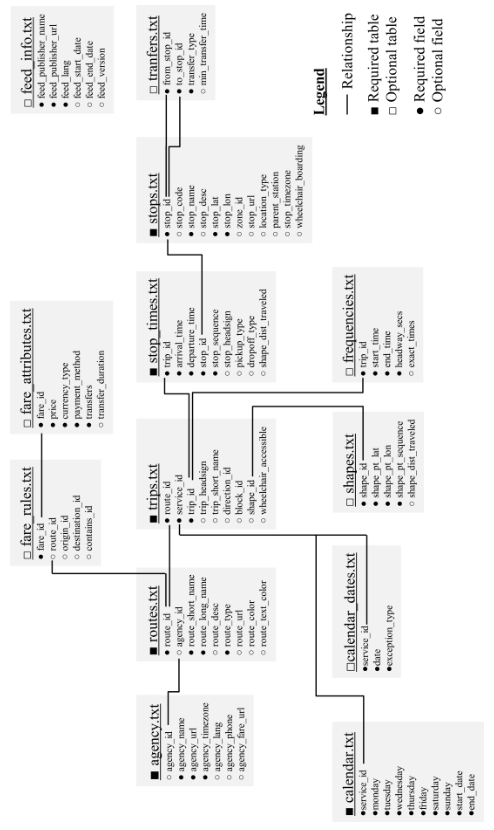
\includegraphics[scale=0.50, angle=270]{imagem/cap2/gtfs_wong.png}
        \source{\citeonline{wong2013}}
        \label{img:2:1}
    \end{figure}
\subsection{GTFS-RT}
On the one hand, the GTFS provides static data of schedules, maps, and fares, on the other hand, 
it neither supplies vehicle positions nor trip updates nor service alerts, natively. The GTFS-RT
is an extension of GTFS, allowing public transportation agencies to provide 
real-time updates about their fleet. Currently,
it supports three types of information served via HTTP and is updated
frequently. Its transmission is based on regular binary files, and there are no 
constraints on how frequently the feed should be updated or retrieved \cite{GTFS-RT}.
The types are listed as:
\begin{itemize}
  \item \textbf{Trip updates} - delays, cancellations, changed routes.
  \item \textbf{Service alerts} - stop moved, unforeseen events affecting a station, route, or the entire network
  \item \textbf{Vehicle positions} - information about the vehicles, including location and congestion level
\end{itemize}

The delays worsen the user experience with the PTN,
GTFS-RT has enabled many researchers to estimate, analyze, and mitigate delays,
due to the temporal features available.
One approach is to stream significant delay changes in
real-time \cite{GTFS-RT_delays_2022-ADWIN}, 
in other words, the user can be notified in real-time with 
schedule deviation. Another approach to mitigate delays is
to collect real-time data and use the temporal series to
predict delays and improve the timetable
\cite{GTFS-RT_delays_2017, GTFS-RT_delays_2022}.

GTFS and GTFS-RT specifications are important in many research fields, such as human mobility. 
Then, it is necessary to comprehend these two specifications to develop a framework to fulfill the GTFS-RT, which could be unavailable, with real-time data from an API combined with GTFS. Finally, our approach uses data structures alike GTFS-RT, as further discussed in Chapter \ref{cap4}.


\section{Complex Networks and Graphs}
In the late 1990s and early 2000s, computational models started to 
deal with huge datasets, which have been only increasing since then. 
In this scenario, complex networks appear to address this issue
based on graph theory designed to model real-world networks, and these models
are suitable to represent relationships and interactions 
between entities through link orientation and labels \cite{barabasiCN}.
Complex networks present compact structures, also called {\em small worlds},
with short distances between nodes, high levels of correlations, and self-organization
\cite{ferber2012}.
The popularization World-Wide Web and its applications, chemistry, drug 
design, natural language processing, and recommender
systems are examples of applications in which complex networks could be used.
To understand a complex network and its metrics, we need to comprehend 
some graphs concepts.

\citeonline{Bacciu_2020} state that "a graph has a compositional nature, being 
a compound of atomic information pieces and a relational nature, as the links
defining its structure denote relationships between the linked entities".
To formally define a graph, the mathematical notation is  \textit{$g = (V_g, E_g, X_g, A_g)$}
where $V_g$ a set of {\em vertexes} and $E_g$ is a set of {\em edges}, or {\em arcs} 
connecting a couple of nodes \cite{graph}. Two more sets, $X_g$ and $A_g$, represent additional information on the node set and the edges set, respectively. In other words, the nodes and edges in some applications have extra features. So, each node $u \in |V_g|$
has a unique feature vector associated therefore, each edge is associated with 
and feature vector $a_{uv} \in A_g$. 

When couples of nodes are ordered, i.e., 
$E_g \subseteq \{\{u,v \} | u,v \in V_g\}$, in a graph, this graph is {\em directed} and its 
edges are {\em oriented}, otherwise the graph is {\em undirected} and its edges 
are {\em non-oriented}. In both directed and undirected graphs, a {\em walk} is a sequence of 
edges that join a sequence of vertexes, a {\em trail} is a walk in which all edges are distinct,
and a {\em path} is a trail in which all nodes are distinct
\cite{williamsonlists}.

\subsection{Public Transportation Networks as a complex network}

The public transportation network is one of the networks that is 
part of the lives of millions of people around the globe, but it 
hides a high complexity degree \cite{ferber2012}.
The PTN can be represented as a {\em directed} graph $G=(V_g,E_g,X_g,A_g)$,
where the set of nodes $V_g$ represents the bus stops and
the set $E_g$ represents the directed arcs that connect different bus stops.
$X_g$ and $A_g$ are the sets of additional information about the nodes 
($V_g$) and the arcs ($E_g$), respectively. Figure \ref{img:2:2} shows $G$. 

    \begin{figure}[H]
     \centering
        \caption{The PTN modeled as the graph $G$}
        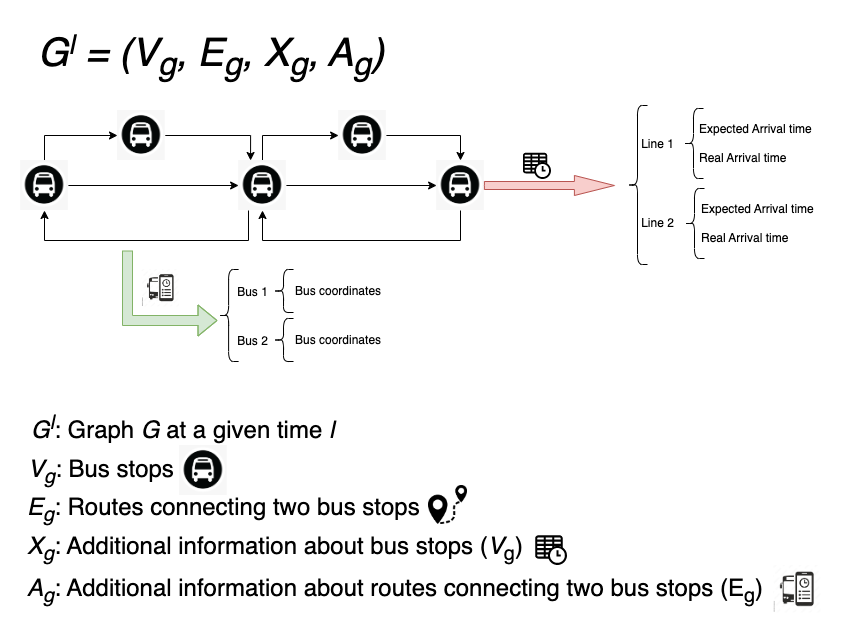
\includegraphics[scale=0.5]{imagem/cap2/final_graph.png}
        \source{The authors}
        \label{img:2:2}
    \end{figure}

$X_g$ contains the bus arrival time on each bus stop in $V_g$. Which is
comprehended as all bus trips that pass by any bus stop $v$ in $V_g$
during a day, for instance. And,
$A_g$ contains the bus entries collected between two sequenced bus stops, $B_x$ and 
$B_{x+1}$. In other words, that is all the information provided by a bus while
traveling through any arc $e$ of $E_g$.


The graph $G$ is a {\em dynamic} graph because the routes change over the days, so the structure of this graph is not fixed.
But, when we approach this graph in a defined time interval, it has a {\em static} topology because the bus stop locations and routes
are not on the same day. Thus, this graph can be
modeled using two data groups, static data, and RT data.
The first group is represented by the GTFS data which is used to generate $V_g$ and
$E_g$ sets, since both sets do not change over the delimited time interval. The second group of data is represented by the real-time bus entries producing $X_g$ and $A_g$ sets, which change over the delimited time interval, meaning
that the traffic will be different on Monday than Tuesday, for example. 


% Nome do capítulo
\chapter{Related work}
% Label para referenciar
\label{cap3}

% Diminuir espaçamento entre título e texto
\vspace{-1.9cm}

% Texto do capítulo

In this Chapter, we present related work identifying delays 
and strategies to mitigate them in public transportation networks.
Also, we approach the issue that GTFS-RT could be unavailable despite
having GTFS and real-time data and how the literature has dealt to
this issue.



\citeonline{delays_bigdata} use the combination of GTFS data and real-time data
to analyze delays in the public transportation network of Rome and Stockholm, 
These cities had divergent data available, resulting in differences in the analysis
used GTFS for the static data. For real-time data,
Rome's data were provided by the Mobility Control Center of Roma Servizi
della Mobilità, but there was no identifier to connect the real-time data
and the static data. So, the link between sets was inferred by comparing the
expected arrival time and the real arrival time within a threshold. The 
results show the average delay for a stop, the average delay for a trip, 
and the average delay for a trip at a stop.

Stockholm's real-time data provided by the Swedish Transportation Administration
and it was easy to link with the static data, unlikely Rome. Also, the real-time
data was composed of real-time updates on routes, disruptions, delays, and 
arrival-departure time of buses, trains, trains, and boats at each stop, 
so characterizing the GTFS-RT specification.
\citeonline{delays_bigdata} used the dataset to examine
three questions:
\begin{enumerate*}
    \item Are the delays in the public transport network spatially
dependent?
    \item What are the factors contributing to delays?
    \item What methods best suit the analysis of large
real-time data streams?
\end{enumerate*}
The first question approach was to calculate the mode and standard deviation
of the delays and apply a simple Moran's I test, which determines a
significant spatial auto-correlation.
The second was tacked using an OLS model in which the average delay is the dependent variable,
and maximum speed, road types, number of lines, and number of lanes are the
independent variables. Finally, regarding the third question, the authors point out 
that spatially aware, computationally intelligent, and machine-learning techniques
to work with this kind of dataset.

We replicated the delay analysis that \citeonline{delays_bigdata} had done in Rome, and we discussed the three questions analyzed with Stockholm's data using
Belo Horizonte data. Belo Horizonte's dataset resembles Rome's because no easy-matching identifier exists. 
Although, we address the issues
with a different approach but also incorporating the key ideas of the algorithm used in Rome, as further discussed in Chapter \ref{cap4}.


Many papers identify delays in public transportation networks using the GTFS-RT 
data, despite the differences in measurement and mitigation of delays, it is
a common approach to model the public transportation network using graph theory.
\citeonline{GTFS-RT_delays_2017} describe that a random delay along legal, physical, or social constraints are the factors that produce delays. To mitigate these factors,
the planners added to the schedule 
a safety margin delay, called schedule padding. 
Furthermore, the schedule padding
is given by the time required to operate on any given segment of the route for
each segment, the padding is the time difference between the fastest and the average time 
of the remaining entries.
A fixed value for schedule padding may heavily influence
the transportation experience by delaying routes without needing to. Then, the takeaway is that
the padding must be proportional to the random delay, which is caused by some unpredictable factors such as: 
traffic conditions, wrecked vehicles, or the number of red lights. 

We molded the public transportation networks using graph theory as well,
and we adapted \citeonline{GTFS-RT_delays_2017}'s concept of schedule padding to 
measure the 
delays and to estimate arrival-departure windows. Because the 
arrival-departure window of a bus to a bus stop depends on whether the bus is
delayed, or on time, or ahead of schedule, which expresses a negative,
neutral, positive padding to the expected arrival time, respectively.

%\citeonline{GTFS-RT_delays_2022}.


\citeonline{routableTimetableGTFS} point out that GTFS' analysis that researchers
have been dealing with could be better addressed using real-time data to enrich 
GTFS data. Because the GTFS is based on schedules, which are projections 
about the services rather than observations.
In other words, the research questions should take into account the events
that interfere with the real composition of the network, the randomness of 
a random complex network. Despite a brief mention of the GTFS-RT
specification, \citeonline{routableTimetableGTFS} reveal one common issue with it,
that is, the non-compatibility of the real-time data and the GTFS. So, they 
propose an algorithm based on the monitoring of vehicles in real-time as their
locations are updated to unify the two datasets. After the data collection,
the algorithm's following steps are: 
\begin{enumerate*}
    \item Delimiting trips and blocks;
    \item Spatial matching and positional error handling;
    \item Determining stop times;
    \item Constructing the retrospective GTFS package.
\end{enumerate*}
Finally, using the enriched GTFS, they demonstrate the usage in Toronto.

%threashold d %
The \citeonline{routableTimetableGTFS}'s algorithm is really interesting; we
approach the real-time data in a very similar outline. 
To delimit trips, we used the vehicle's current distance en route instead of 
the headsign. To do spatial matching and positional error handling, they used
Open Source Routing Machine's map-matching algorithms to match entries to 
bus stops, we opted for keeping a low-coupling architecture using the 
Postgis and GTFS. 
For determining stop times, we used the same approach of estimating time
by linear interpolation from the surrounding vehicle reports, but we propose 
a different heuristic to choose the reports to interpolate.
The architectural decisions we made and our justifications are further explored in
the following chapter, Chapter \ref{cap4}.

Given the state-of-the-art literature discussed in this chapter,
this dissertation contributes to GTFS and GTFS-RT because we present
a tool to link GTFS with real-time data in cities where GTFS-RT is unavailable, allowing analysis such as delay analysis. Then, we contribute to 
delay analysis due to the reproduction of questions using the proposed framework.

% Nome do capítulo

\chapter{PondiônsTracker}
% Label para referenciar
\label{cap4}

% Diminuir espaçamento entre título e texto
\vspace{-1.9cm}

% Texto do capítulo
In this Chapter, we present \textit{PondiônsTracker}\footnote{Available at \url{https://github.com/Pongelupe/PondionsTracker/}}, 
which is a framework to enrich
GTFS data with real-time data enabling { \em collecting } and { \em integrating }. 
The name \textit{PondiônsTracker} is a small gag from the sonority of the expression{ \em bus stop}
when pronounced in Portuguese with the accent from Minas Gerais, and its architecture is divided into two components: 
the data module, and
the integration module 
as shown in the architecture diagram from Figure \ref{architecture:diagram}.
In the following Sections of this Chapter, we present the entities used by the components,
then we deep dive into each component and finish presenting \textit{PondiônsTracker-BH}.


\begin{figure*}[h]
     \centering
        \caption{\textit{PondiônsTracker}'s architecture diagram}
        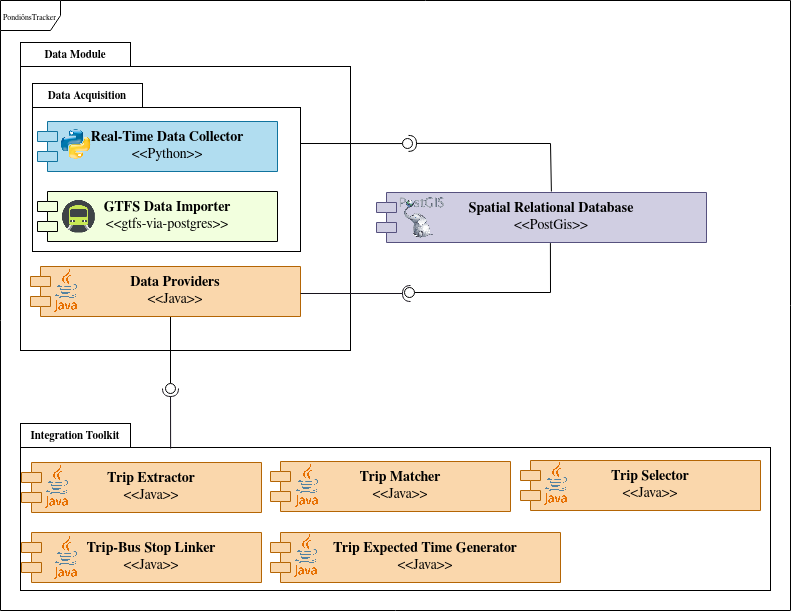
\includegraphics[width=.95\textwidth]{imagem/cap4/arq-pondionstracker.drawio.png}
        \source{The authors}
        \label{architecture:diagram}
\end{figure*}

{ \em Loose coupling} is the key design principle of \textit{PondiônsTracker} architecture to work with as many cities as possible, and this can be achieved by smaller software components that can be 
replaced or extended and still work with the other components with few adjustments, 
because the behaviors of the main components are defined in interfaces, so an object-oriented language as Java suits this scenario.
The major external dependency is the \textit{PostGIS}\footnote{Available at \url{https://postgis.net/}}
database, which provides spatial functions and stores the data.  


\section{Entities}
\begin{figure}[h]
     \centering
        \caption{Entities Class Diagram}
        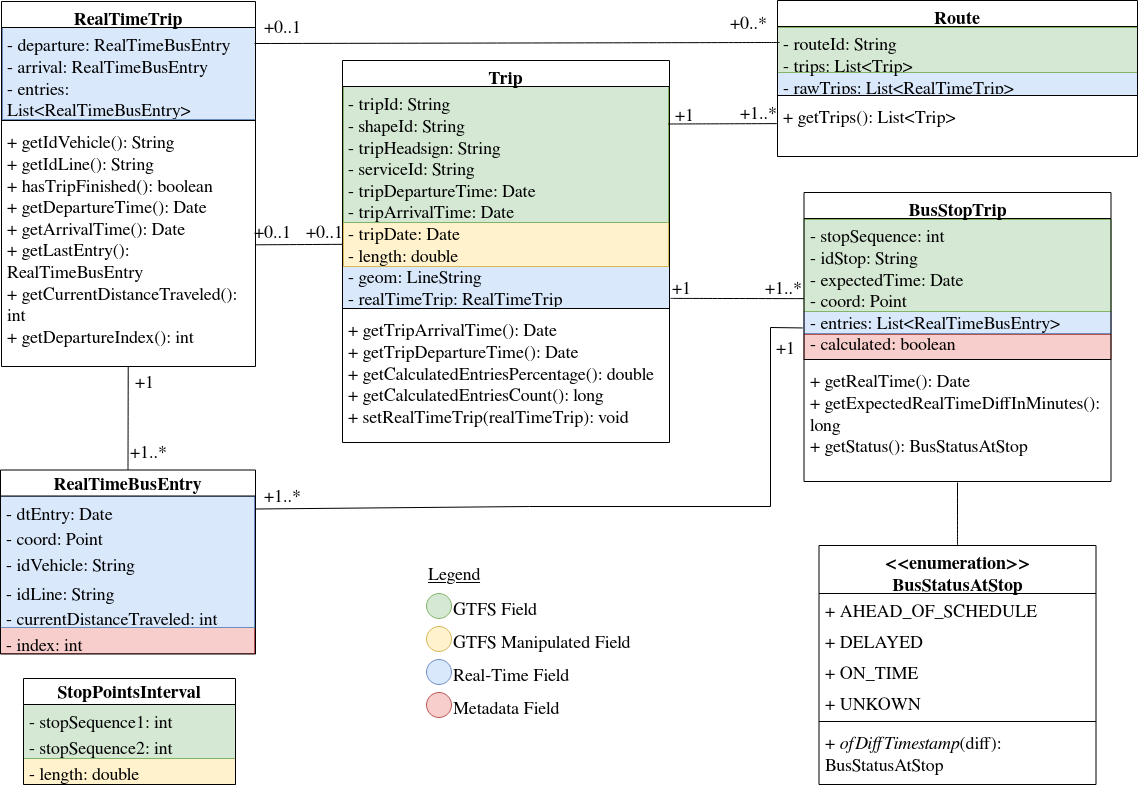
\includegraphics[width=\textwidth]{imagem/cap4/entitiesCD.png}
        \source{The authors}
        \label{cdEntities}
\end{figure}

In this Section, we present PondiônsTracker's entities used in all components, the entities
mix three types of fields: fields from the GTFS specification, fields to represent the 
real-time data and some auxiliary fields, Figure \ref{cdEntities} presents the entities 
class diagram with the getters and setters suppressed to improve the readability.
The fields highlighted in green are from the GTFS, and those highlighted in yellow are not originally from the given entity, but they are easily obtained by 
manipulating other fields, such as the \textit{Trip}'s $geom$ and \textit{BusStopTrip}'s
$coord$ which are spatial data from $shape\_id$, $stop\_lat$ and $stop\_lon$, respectively.
Finally, the fields highlighted in blue are from the real-time data,
and those highlighted in red were designed to store metadata produced during the components' execution.


The \textit{Route} and \textit{Trip} entities are defined at the GTFS specification, 
and we enriched both with more fields, the $rawTrips$ 
was added to the \textit{Route} to link with all the related raw 
real-time trips collected. Four new fields were introduced to the 
\textit{Trip}, two in yellow and two in blue, the yellow couple represents the spatial, 
in which $length$ represents the $geom$ length, that is a \textit{LineString} with
the bus stops are linked by the path programmed, in meters. Furthermore, in the blue couple,
$realTimeTrip$ corresponds to the real trip of a scheduled trip, which is a zero or one 
relationship, because
one $Trip$ can have at most one related \textit{RealTimeTrip}, but it also is unavailable, leading to a null reference. 
And $busStopSequece$ is a \textit{List} of all stops of this trip ordered by its $stop_sequence$, in other 
words, a list of \textit{BusStopTrip}.

The \textit{BusStopTrip} works as an entity that merges two GTFS's entities: \textit{stop\_times} and \textit{stops}. The first brings $stop\_sequence$, $stop\_id$, and $departure\_time$ that could be null
depending on the local GTFS. And, \textit{stops} provides the spatial information achieved 
using the $stop\_id$. The field $entries$, which is highlighted in blue, represents all the \textit{RealTimeBusEntry} related to this stop, which may be even zero, in other words, it is a
list containing every bus that was around this stop. Finally, the $calculated$ field in red
is a flag representing that this \textit{BusStopTrip} has no actual entry related to it, so an artificial 
entry was created and associated with this stop, as further explained in Section \ref{sub:integration}.
Finally, the method \textit{getStatus} gets the \textit{BusStatusAtStop} of the current \textit{BusStopTrip}, and this operation enables the delay analysis.

Then, for every bus positioning, around or not around a bus stop,
is entry from \textit{RealTimeBusEntry}, which is the entity that summarizes 
all \textit{PondiônsTracker}'s real-time required blue fields in a group of five as 
follows:
\begin{enumerate*}
    \item $dt\_entry$: Timestamp of the occurrence;
    \item $coord$: The location of the occurrence. Mainly given by lat/lon coordinates;
    \item $id\_vehicle$: A identifier for the vehicle executing the trip;
    \item $id\_line$: A identifier for the route/trip being executed;
    \item $current\_distance\_traveled$: The current distance traveled in a trip.
\end{enumerate*}
And a \textit{RealTimeTrip} is achieved by ordering the entries by its $dt\_entry$ 
then group them by $id\_vehicle$, which is the concept that a single bus can only travel
a single trip at a time. Finally, the field in red $index$ represents the position of an
entry in a trip.


\section{Data Module}
The Data Module's main goal is to encapsulate 
operations of the \textit{PostGIS} from the other components. 
There are three artifacts inside this module, 
\textit{DataImporter},
\textit{RealTimeDataCollector},
and \textit{DataProviders}, 
the first two components encapsulate writing, and the last encapsulate reading.
Also, there are two \textit{DataProviders}, one that works with GTFS data and the
other works with real-time data, \textit{GTFSProvider} and \textit{RealTimeProvider},
respectively.

\subsection{GTFS Data Importer}
The \textit{GTFS Data Importer} is a component that imports the GTFS data to the \textit{Postgis}
and creates the basic structure needed. So, given an instance of \textit{Postgis} running 
in a cloud service or local or dockerized environment, for instance, the first step is to 
execute the \ac{DDL} required, which is defined at \textit{schema.sql} that is a \ac{SQL} file 
located at $scripts/sql/$. 
\textit{schema.sql} defines two tables, and the first is called 
{\em  real\_time\_bus} is a table to store the real-time data. In other words, each row is
an instance of a \textit{RealTimeBusEntry}. And, for this table, there are two indexes,
one is over $dt\_entry$ and the other over $dt\_entry$ combined to $id\_vehicle$, 
they are designed to improve the performance of the queries executed by the \textit{Data Providers},
further explained in Subsection \ref{sub:dataProviders}. Figure \ref{fig:rmRTB} shows its relational model.

\begin{figure}[h]
\centering
\begin{minipage}[t]{.5\textwidth}
  \centering
  \caption{{\em  real\_time\_bus}'s \\relational model}
  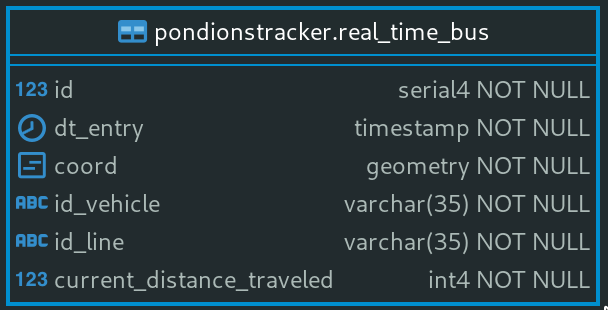
\includegraphics[width=.99\linewidth]{imagem/cap4/real_time_bus_ER.png}
  \source{The authors}
  \label{fig:rmRTB}
\end{minipage}%
\begin{minipage}[t]{.5\textwidth}
  \centering
  \caption{{\em  shapes\_summarized}'s \\relational model}
  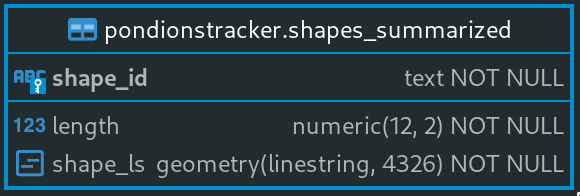
\includegraphics[width=.99\linewidth]{imagem/cap4/shapes_summarized_ER.png}
  \source{The authors}
  \label{fig:rmSS}
\end{minipage}
\end{figure}

Figure \ref{fig:rmSS} shows the relational model of the second table created, called {\em  shapes\_summarized} and is an auxiliary table 
that stores the geometric type $LineString$ and its length for all trips. 
This table is needed because the tool used to import the GTFS data does not
provide this structure or a similar one. The tool used is the \textit{gtfs-via-postgres} 
\footnote{Available at \url{https://github.com/public-transport/gtfs-via-postgres}},
an open-source solution to import static data that Google recommends. It takes as input the
GTFS files, which could be in the $.txt$ or $.csv$ format, and create a new table in the database for each
entity. 

Finally, the last step to fully initialize the database is to execute an SQL script that populates
the table {\em  shapes\_summarized}, which is \textit{shapes\_summarized\_populate.sql}
and it is located in the same folder as \textit{schema.sql}.
This SQL script takes the \textit{shapes} table grouped by the $shape\_id$
as input to the \textit{PostGIS}'s function { \em ST\_MakeLine} that produces a $LineString$ from the given points.

We provide a{ \em shell} script that executes all the steps described previously, this script is 
called $init.sh$, and it is in the folder $scripts$. This script takes two inputs: 
the first argument is the path to the folder where the GTFS's files are located, and 
the other argument is the schema name that \textit{gtfs-via-postgres} is going to import to.
$init.sh$ uses \textit{PostGIS}'s environment variables
\footnote{Available at \url{https://www.postgresql.org/docs/current/libpq-envars.html}}
to connect to the database, then execute three commands. The first loads \textit{schema.sql},
the second uses \textit{gtfs-via-postgres} to import the GTFS, and the third executes the 
\textit{shapes\_summarized\_populate.sql}.


\subsection{Real-Time Data Collector}
The \textit{Real-Time Data Collector} is the component responsible to 
collect the real-time data and insert it into {\em  bus\_real\_time},
encapsulating the writing into the database. In other words, this component will incorporate the data 
from real-time traffic \ac{API} provided by some external source into the table, such as traffic agencies.
Regarding extensibility, {\em bus\_real\_time} can be enriched with more data, 
instant speed, and direction, for instance.

The Real-Time Data Collector may be implemented in any language since
it must adapt to each real-case scenario to insert valid entries into the table
because it depends on the local city provider.
To illustrate a record, an API provides the following data:
A bus $b$ of line 123 is at a bus stop
near a drugstore and has already traveled 3 km on its route at 4 p.m.
The corresponding entry would be:
\begin{enumerate*}
  \item $dt\_entry$ as 16:00;
  \item $coord$ as the point composed by the latitude and longitude of the 
  bus stop near a drugstore where the $b$ is;
  \item $id\_vehicle$ as the $b$'s vehicle id;
  \item $id\_line$ as 123;
  \item $current\_distance\_traveled$ as 3000, which is 3km transformed to meters.
\end{enumerate*}
And the $id$ is generated and managed by the database.


\label{sub:dataProviders}
\subsection{Data Providers}

\begin{figure}[h]
     \centering
        \caption{Data Providers Class Diagram}
         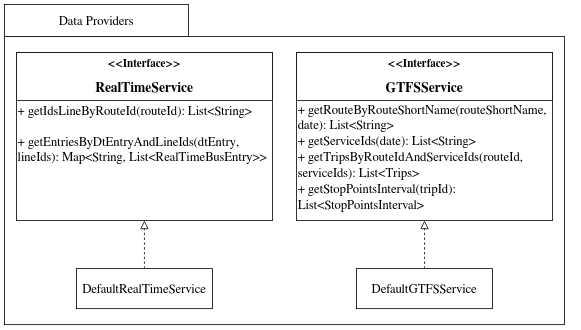
\includegraphics[width=.9 \textwidth]{imagem/cap4/dataProviderED.drawio.png}
        \source{The authors}
        \label{cdProviders}
\end{figure}

To isolate the access to the \textit{PostGIS}, the Data Providers are designed to 
supply all the data  required in other modules. Figure \ref{cdProviders} represents the class diagram for these components, then
it is composed of two interfaces: \textit{RealTimeService} and \textit{GTFSService}, which represent the real-time data 
and the GTFS data, respectively. 
Also, each of these interfaces has a default implementation, 
the \textit{RealTimeService} implementation is \textit{DefaultRealTimeService} 
and the \textit{GTFSService}'s default implementation is given by \textit{DefaultGTFSService}. 
The Data Providers are available at the Maven Repository and can be accessed by adding the 
following dependency to a \textit{pom.xml} in a Java 17+ project.
\begin{lstlisting}[language=XML]
		<dependency>
			<groupId>br.pondionstracker</groupId>
			<artifactId>data-module</artifactId>
			<version>1.0.0</version>
		</dependency>
\end{lstlisting}

The \textit{DefaultRealTimeService} implements the two methods defined by the interface. 
The first is called \textit{getIdsLineByRouteId}, It takes a route id
as input and produces a list containing all the line identifiers related to the given route, 
the default implementation is to return a list of a single item, which item is the inputted route id.
In other words, this method establishes the relationship between the two datasets heavily dependent
on each city context. Although this method is likely to be overridden, 
the default implementation assumes that the RT provider will use the $route\_id$.

The second method is called \textit{getEntriesByDtEntryAndLineIds}, it takes a target date and 
the $id\_line$s as input and produces a \textit{java.util.Map} whose key is $id\_vehicle$ and value
is a list of entries related to the $id\_vehicle$. So, the main idea, which is also implemented by the  
\textit{DefaultRealTimeService}, is to retrieve all the entries from a day of some lines ordered by $dt\_entry$ grouped by 
$id\_vehicle$, the \textit{TripExtractor} is going to take advantage of this grouping, 
as further approached in Subsection \ref{sub:2}.

The \textit{GTFSService}'s default implementation is given by \textit{DefaultGTFSService} 
which implements the four methods defined. The first is called \textit{getRouteByRouteShortName},
it takes a $route\_short\_name$ and a target date as input and produces a 
\textit{java.util.Optional} of a 
$Route$, the \textit{Optional} is going to be filled if the $route\_short\_name$ exists at the given date,
empty otherwise. The default implementation fills the $trips$ object using two other methods available,
\textit{getServiceIds} and \textit{getTripsByRouteIdAndServiceIds}. The method called \textit{getServiceIds}
takes a target date as input and retrieves all the valid $service\_id$s at the given date, that is, all the 
available services for that day of the week.

The method called \textit{getTripsByRouteIdAndServiceIds} takes a $route\_id$ and a \textit{List} of 
$service\_id$ as input and produces a \textit{List} of trips that is the schedule of each trip of that route. 
The default implementation retrieves the following fields: $trip\_id$, $shape\_id$, $service\_id$, 
$trip\_headsign$, $shape\_ls$, and $length$. Then, for each trip, the $busStopSequence$ is filled with
its stop sequence, stop id, expected time, and the bus stop coordinates. 
Finally, the last method is called \textit{getStopPointsInterval}, it takes a $trip\_id$ as input and 
produces a \textit{List} of \textit{StopPointsInterval}. That is, the trip's bus stops in sequence and
the distance between a couple of stops.



\section{Integration Module}
\label{sub:integration}
The Integration Module's main goal is to provide functions and methods to 
work with the transit data previously collected using the {\em GTFSService and RealTimeService}.
So, this module exposes seven interfaces, which are \textit{TripExtractor}, 
\textit{TripMatcher},
\textit{TripBusStopLinker},
\textit{TripSelector},
and \textit{TripExpectedTimeGenerator} as shown in Figure \ref{cdIntegration}. 
In the following Subsections, we get into details of the interface contracts
and its{ \em default} implementation. In the last Subsection, we approach the 
\textit{Drivers}. Finally, all the interfaces and their default implementation are  
available at the Maven Repository and can be accessed by adding the 
following dependency to a \textit{pom.xml} in a Java 17+ project.
\begin{lstlisting}[language=XML]
		<dependency>
			<groupId>br.pondionstracker</groupId>
			<artifactId>integration-module</artifactId>
			<version>1.0.0</version>
		</dependency>
\end{lstlisting}


\begin{figure}[t]
     \centering
        \caption{Integration Module Class Diagram}
        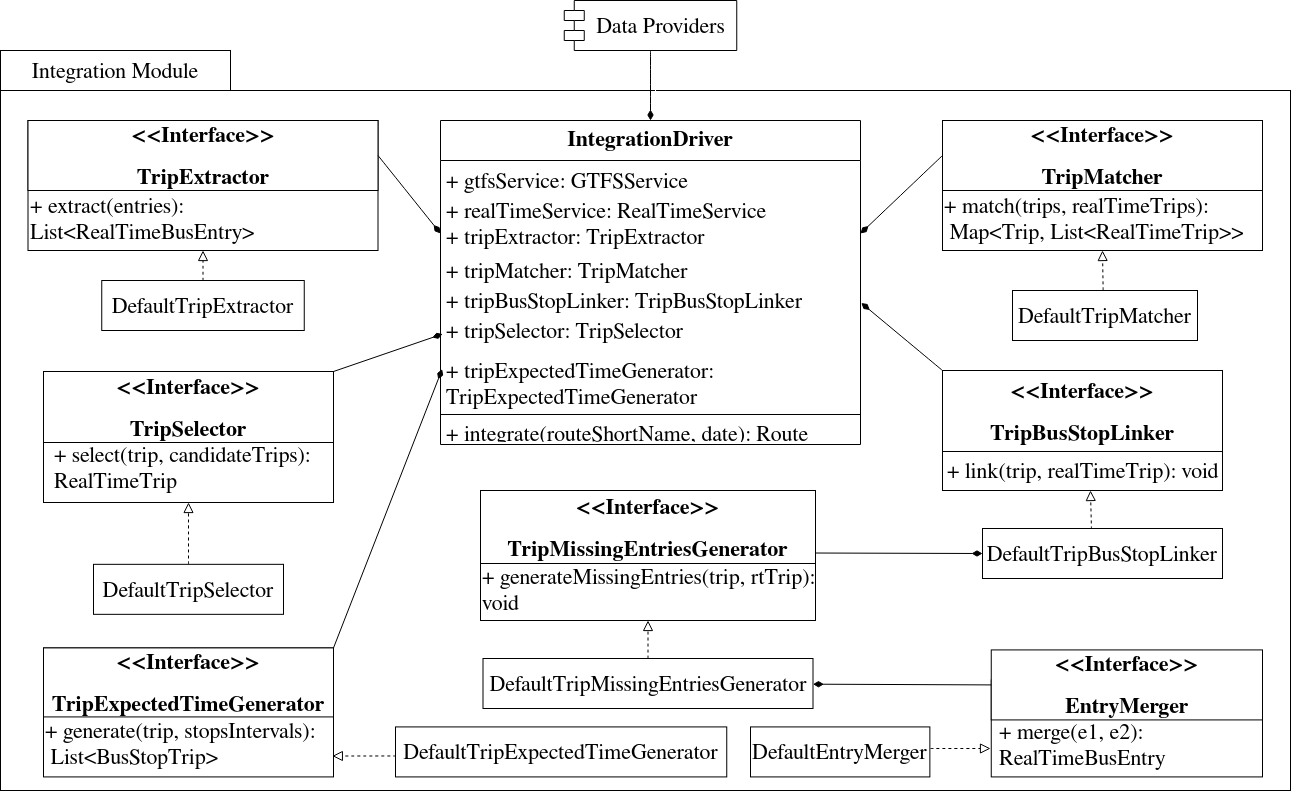
\includegraphics[width=\textwidth]{imagem/cap4/integrationModuleCD.png}
        \source{The authors}
        \label{cdIntegration}
\end{figure}


\subsection{Trip Extractor}
\label{sub:2}
The \textit{TripExtractor} is an interface that declares one method which is called
\textit{extract} that takes a \textit{List} of $RealTimeBusEntry$ as input and produces
a \textit{List} of $RealTimeTrip$. This component's main goal is to extract the trips from
entries because the data from the real-time API may not have a direct link to the GTFS, 
which leads to scenarios where APIs supply more data than the scheduled trips.
In other words, a trip represents a {\em trail} in the graph.
In addition, the APIs might return some unwanted trips, such as the displacement 
from the bus garage to a bus stop, and the other way around,
the{ \em default} implementation does not apply any strategy to filter out these 
trips. The implementation is defined in Algorithm \ref{alg:extract} and depends on three premises:
\begin{enumerate*}
    \item The entries must be from the same $idVehicle$;
    \item The entries must be sorted by $dtEntry$ in order to preserve their chronology;
    \item The $currentDistanceTraveled$ can only increase for the same trip.
\end{enumerate*}

After postulating these premises, it is iterated over entries, then for each entry,
it $currentDistanceTraveled$ is compared with a temporary variable $d$ defined on
line \ref{alg:extract:d}. If the entry's $currentDistanceTraveled$ is{ \em lower} 
than $d$, represented by the $if$ command on 
line \ref{alg:extract:if}, it implies that a trip has just finished due to the third premise at 
this point, it is assigned the $previousEntry$ to the $arrivalEntry$, on
line \ref{alg:extract:arrival}.
Otherwise, when $d$ is greater than or equal to the entry's 
$currentDistanceTraveled$ and the $arrivalEntry$ is still null, and the entry might be the $departureEntry$ or an intermediate entry.
Finally, after iterating over all entries, it is added to $trips$ the 
last trip that is composed of the variables $departureEntry$ and $previousEntry$,
the $previousEntry$ contains the{ \em last} entry of the List inputted, then 
$trips$ are returned.

\begin{algorithm}[t]
\caption{\textit{DefaultTripExtractor}'s implementation}\label{alg:extract}
\begin{algorithmic}[1]
\State $trips \gets [ ]$
\State $d \gets 0$ \Comment{currentDistanceTraveled}
 \label{alg:extract:d}
\State $departureEntry \gets null$
\State $arrivalEntry \gets null$
\State $previousEntry \gets null$
\For{$i\leq entries.length; i++$} 
    \State $entry \gets entries[i]$
    \If{$entry.currentDistanceTraveled\geq d$}
    \label{alg:extract:if}
        \If{$arrivalEntry \neq null$}
            \State $trips.add(new Trip(departureEntry, arrivalEntry))$
            \State reset temp vars to initial state
        \Else
            \State $d \gets entry.currentDistanceTraveled$
        \EndIf
        \If{$departureEntry$ is null}
            \State $departureEntry \gets entry$
        \EndIf
    \Else
        \State{$arrivalEntry \gets previousEntry$}
        \label{alg:extract:arrival}
        \State $d \gets entry.currentDistanceTraveled$
    \EndIf
    \State{$previousEntry \gets entry$}
\EndFor 
\State $trips.add(new Trip(departureEntry, previousEntry))$
\State return trips
\end{algorithmic}
\end{algorithm}

Algorithm \ref{alg:extract}'s output is all the trips delimited by its vehicles 
and timestamps, but they are not linked to a route yet. 
The complexity of this algorithm is $O(n)$, in which 
that $n$ corresponds to entries generated by a single bus in an interval, and it is necessary to iterate once over $n$ to delimit the trips.
Despite the $O(n)$ 
complexity, it is worth noticing that $n$ corresponds to entries produced by a single 
bus in an interval, then Algorithm \ref{alg:extract} {\em might} be executed over a hundred times
for a single day of observation, for instance.

\subsection{Trip Matcher}
The \textit{TripMatcher} is an interface that declares one method, which is called
\textit{match} that takes two \textit{Lists} as input, one of $Trip$ and the other
of $RealTimeTrip$. Then, it produces a \textit{Map} of all $RealTimeTrip$s related to a 
$Trip$. So, this component is responsible for linking the static to the real-time data,
the{ \em default} implementation tries to unify the scheduled block with the 
delimited trips from real-time data by comparing \textit{Trip}'s 
and \textit{RealTimeTrip}'s $departureTime$. 
To do so, the key idea is to iterate over all the trips
from $trips$, and for each scheduled trip, all real-time trips 
that $departureTime$ is within an interval $i$ is reserved to the block otherwise, it is discarded. 

This interval represents the trip's maximum initial shifting 
and is a required argument to instantiate \textit{DefaultTripMatcher}, which is 
used to initialize the final field, $maxTripInitialShifting$. 
That is a minute interval that works to mitigate minor deviations from
the schedule at the start of  a trip that is likely to happen due to real-time data 
unpredictability. 
Then, $maxTripInitialShifting$ works both for delayed and ahead-of-schedule lefts because 
it is taken into account in an absolute value, 
for instance, when $maxTripInitialShifting=5$ it matches a trip that is 5 minutes delayed or 5 minutes ahead of schedule. Finally, to exactly match on-time trips, $maxTripInitialShifting = 0$. 

\textit{DefaultTripMatcher}'s complexity is $O(rt)$, in which $r$ is the size of $trips$
and $t$ is the size of $realTimeTrips$. $r$ is constant because its source
is the GTFS data, and $t$'s size is unstable due to the real-time data, 
so $\Omega(n^2)$, or even lower when $r > t$.
Despite having the lowest complexity, lower than $\Omega(n^2)$, this scenario
is undesired because it represents that there are more scheduled trips than 
trips collected, which indicates some degree of information loss. 
When $r = t$, it represents the best-case scenario regarding information
recovery because there is the same number of scheduled trips and trips collected,
corresponding to a complexity of strictly at $\Omega(n^2)$. In most cases, $r < t$ is due to
the unwanted trips, then $\Theta(rt)$.


\subsection{Trip Selector}
The \textit{TripSelector} is an interface that declares one method, which is called
\textit{select} that takes a $Trip$ and \textit{List} of $RealTimeTrip$ as input 
and produces a \textit{List} of $RealTimeTrip$. This component's main goal is to
{\em select} the $RealTimeTrip$ trip that better fits the $Trip$.
The default implementation selects the $RealTimeTrip$, which has the latest 
$departureTime$ that fills the two following conditions:
\begin{enumerate}
    \item The last entries $dtEntry$ must be after the $departureTime$;
    \item The trip must have traveled at least a $tripMinPercentageTraveled$ percentage of the \textit{Trip}'s $length$.
\end{enumerate}

$tripMinPercentageTraveled$ is a required argument to instantiate 
\textit{DefaultTripSelector} and it represents the \textit{RealTimeTrip}'s minimum percentage traveled of the \textit{Trip}. In other words, it is a parameter that
defines the concept of a completed trip. \textit{DefaultTripSelector} has 
a complexity of $O(n)$ because it iterates over the candidate real-time trips
and selects the trip with the latest $departureTime$ that fills the preconditions defined above.

It is necessary to select the candidate trip because there are some unwanted trips, such as the displacement from the bus 
garage to a bus stop and the other way around. Among all trips, some
unfinished trips get distinguished by not going through all bus stops on a route
due to many factors, such as
\begin{enumerate*}
  \item Bus breaking down.
  \item The bus' communication system is malfunctioning.
  \item A bus' last entry recorded is still en route.
\end{enumerate*}

\subsection{Trip-Bus Stop Linker}
The \textit{TripBusStopLinker} is an interface that declares one void 
method which is called \textit{link} that takes a $Trip$ and a $RealTimeTrip$ as input
and fills each $entries$ set from $Trip$'s $busStopSequence$.
In other words, this component's main objective is to link 
a real-time trip to the bus stop from a scheduled trip,
which binds static data alongside real-time data. 
Although this component can be used alone,
and it was designed to work with the output of the previous component
to enrich the trips with some initial route information.
The default implementation assumes that the $RealTimeTrip$ have
been around every bus stop from their route. 

Furthermore, in the context of the default implementation, 
the entry is considered to be around the bus stop if it is {\em at} or
{\em near}. Matching the entry and the bus stops is not a simple task due to GPS position errors caused by the
lack of synchronization between the datasets. 
These errors are pretty common 
and well-expected, it is unlikely that the entry's $coord$ is exactly 
{\em at} the bus stop for many reasons, such as the bus broke or was simply too fast, and the dataset missed capturing the instant. 
These issues are reported in 
\citeonline{routableTimetableGTFS}, and 
we adopted their concept of a distance threshold between an entry and the bus stop for positioning, and from here, we are going to reference this threshold as $d_t$, so an entry 
within $d_t$ is considered {\em at} a bus stop. Figure \ref{img:4:3} illustrates an
entry within $d_t$, and Figure \ref{img:4:emptyset} shows a couple of entries, $e_1$ and $e_2$, which are not 
within $d_t$, for instance.


\begin{figure}[h]
     \centering
        \caption{Entries and $d_t$ representations}
        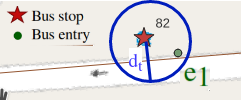
\includegraphics[scale=.65]{imagem/cap4/entriesDT.drawio.png}
        \source{The authors}
        \label{img:4:3}
\end{figure}

\begin{figure}[h]
     \centering
        \caption{Empty set of entries}
        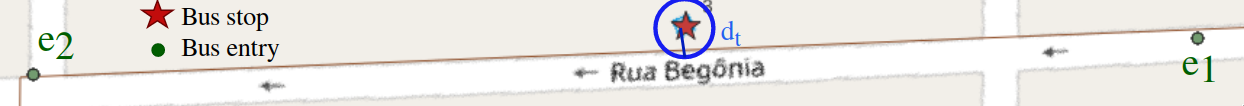
\includegraphics[width=\textwidth]{imagem/cap4/9202_empty_set.png}
        \source{The authors}
        \label{img:4:emptyset}
\end{figure}

So, the \textit{DefaultTripBusStopLinker} associates each bus stop from 
the scheduled trip with a set of entries there is within $d_t$.
However, an entry that is within $d_t$ is not necessarily 
part of the set because a single entry might be within $d_t$
of more than one bus stop. 
For instance, one avenue has a couple of bus stops on the same route
which are on opposite sides, and consequently, 
they are in different directions of the route. 
One entry between these two bus stops is related 
to only one of them, one bus cannot be at two stops simultaneously. Thus, the key idea is to match entries and bus
stops within $d_t$ and in the same direction as the route.

The default implementation key idea is to iterate over $Trip$'s $busStopSequence$
and for each bus stop $s_x$ it is searched for all the valid entries within $d_t$, then scanning the $RealTimeTrip$'s $entries$ set.
The three following premises are required to relate an entry $e$ to a bus stop $s_x$:
\begin{enumerate}
  \item an entry $e$ can be associated with only one $s_x$;
  \item a $s_x$ can be related to more than one entry $e$;
  \item a $s_x$ can be related to zero entries.
\end{enumerate}

The complexity of this operation is $O(n \log_k)$, in which
$n$ is the number of stops in a trip and $k$ is the size of entries of
the real-time trip. The first premise postulated assures the complexity of $\log_k$ when 
iterating through the entries set because the search for a stop $s_x$ starts at 
the index of the last entry related to a previous bus stop.

%\label{sub:generator}
%\subsection{Trip Missing Entries Generator: Entry Merger and Entry Merger Selector}

After executing the previous operation, each set of entries 
related to each bus stop should have {\em at least} one entry, 
but sometimes, the set is empty. 
And this does not imply that the bus has not been around a stop on the trip, 
it might be only a GPS positioning error. For example, if a bus is at a
certain speed, then it passes by a bus stop without stopping because there
are not any boarding nor landing at that given stop. Consequently, the
set of entries will be empty, and the third premise represents it. 
In other words, we know 
that the bus had been around to the stop, but there was not a single entry
close enough, as $e_2$ from Figure \ref{img:4:emptyset}. 
In this scenario, the \textit{DefaultTripBusStopLinker} executes an extra step
to generate an artificial entry at the stop with an empty set using the 
closest couple of entries, described by interface \textit{TripMissingEntriesGenerator}.

The \textit{DefaultTripMissingEntriesGenerator} design is to iterate over each 
bus stop $s_k$ from $Trip$'s $busStopSequence$ with no entry related to it. 
Then, each $s_k$
is going to be linked to a new artificial entry $e_g$ that is going to be
generated by the merge of a couple of entries. The \textit{EntryMerger} is the component
in charge of merging two entries, the strategy behind it is to execute a linear interpolation
between the two entries $coords$ and other attributes, which is a simple operation
whose complexity is \textit{constant}. To illustrate, if the merged entry $e_{(n-1, n)}$
is the product of $e_{n-1}$ and $e_n$ then it is going be as shown in Table \ref{tab:merger}.

\begin{table}[h]
\centering
\caption{Example of merge of $e_{n-1}$ and $e_n$ } 
\begin{tabular}{|l|c|c|c|c|}
\hline
\multicolumn{1}{|c|}{} & $dt\_entry$    & $coord$    & \multicolumn{1}{l|}{$id\_vehicle$} & \multicolumn{1}{l|}{$current\_distance\_traveled$} \\ \hline
$e_{n-1}$                & 10:00 &  coord $e_{n-1}$         & 1     &    5000     \\ \hline
$e_n$                & 10:02  & coord $e_{n}$ &               1    & 5100                   \\ \hline
$e_{(n-1, n)}$                & 10:01 & coord $e_{(n-1, n)}$ &    1               & 5050                 \\ \hline
\end{tabular}
\source{The authors}
\label{tab:merger}
\end{table}


The task of selecting which couple is going to be merged is complex as well and
it is performed by the interface \textit{EntryMergerSelector}.
For instance, given a bus stop $s_n$, in which $n$ represents the sequence of that stop on
the trip and $s_n$ has no entry related to it,
then an artificial entry $e_g$ is going to be generated by the merge of two other entries. 
In the default implementation,
the first step in choosing these entries to merge is to comprehend that one is before and 
another is after $s_n$ to guarantee that the bus had passed by the stop, and,
the fact that multiple entries may exist in between. 
So, the key idea is to search for the two closest entries to $s_n$
from an interval of entries ranging from a {\em Lower Bound Entry} 
and an {\em Upper Bound Entry}.


    \begin{figure}[h]
        \centering
        \caption{A more complex scenario of no entries within $d_t$}
        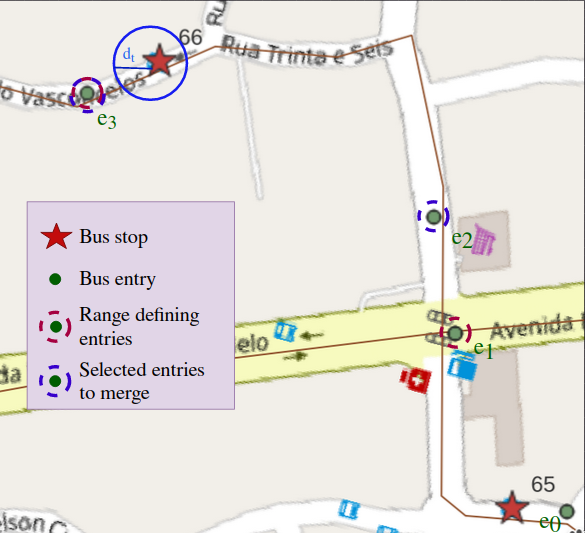
\includegraphics[scale=0.5]{imagem/cap4/9202_hard.png}
        \source{The authors}
        \label{img:4:4}
    \end{figure}

On the one hand, the {\em Lower Bound Entry} must be the entry with the latest $dt\_entry$
related to any other $s_{x}$ where $x < n$, that is the representation of 
the latest entry before $s_n$. On the other hand, the {\em Upper Bound Entry} 
must be the entry with the earliest $dt\_entry$ related 
to any other $s_{x}$ where $x > n$, which is the representation of 
the earliest entry after $s_n$. Figure \ref{img:4:emptyset} represents a scenario 
where the interval contains only the boundary entries so that they will be merged. Figure \ref{img:4:4} pictures a more complex scenario
in which to generate an entry related to the bus stop $S_{66}$ is needed to evaluate
the following set: $E = \{{e_1, e_2, e_3}\}$, then choose the two nodes with
the lowest distance to $S_{66}$, that are $e_2$ and $e_3$. In this case,
the {\em Lower Bound Entry} is $e_1$, and the {\em Upper Bound Entry} is $e_3$.

The \textit{DefaultTripMissingEntriesGenerator} complexity is $O(2n + c)$ because
the complexity of finding out each boundary entry is $O(n)$ and 
the merge algorithm adds the constant $c$. Then, the final complexity to 
generate an entry associated with a bus stop is $O(2n)$, consequently,
the \textit{DefaultTripBusStopLinker} complexity is $O(n \log n + 2n)$ which 
is the sum of the complexity of the two steps.




\subsection{Trip Expected Time Generator}
The \textit{TripExpectedTimeGenerator} is an interface that declares one method, which is called
\textit{generate} that takes a $Trip$ and \textit{List} of $StopPointsInterval$ as input 
and produces a \textit{List} of $BusStopTrip$, The default implementation generates the expected stop time using
the average route speed with the complexity of $O(n)$ where $n$ is
the number of stops. 

The \textit{DefaultTripExpectedTimeGenerator}'s key concept is that the stop times are incremental in the trip
and are incremented at each stop. In other words, for each bus stop, we increase to the initial $arrival\_time$ some time interval until the point it gets to the $departure\_time$ at the last bus stop. 
This time interval referenced is calculated for a bus stop 
$S_n$ using two values: 
the distance between $S_{n-1}$ and $S_n$ and the average trip speed.
The latter is constant due to the length of the trip and 
the required $arrival\_time$ and $departure\_time$ fields, which are used to infer the total
route duration, then the average trip speed is the division of the route length by the trip duration.

Calculating the distance between each $S_{n}$ and $S_{n+1}$ is not as straightforward as it looks
because of the route, the distance is not as simple as a line connecting these stops, and the paths
may contain turns and direction changes. An approach to this issue is the usage of 
Open Source Routing Machine's routing algorithms are similar to those used by \citeonline{routableTimetableGTFS} for map-matching. We relaid on the GTFS data, the {\em  shapes\_summarized} SQL table, 
and the following \textit{PostGIS} functions:
$ST\_LineLocatePoint()$, $ST\_Length()$ and $ST\_LineSubstring()$. 
Our approach consists of grouping and ordering the stops by couples using the $stop\_sequence$, 
consequently generating a route segment connecting each couple stop whose distance
is used to calculate the time needed to travel this segment.



Figure \ref{img:4:5} represents a bus stop couple for each record in which the first two 
columns indicate origin and destination stops, and the third and fourth columns are the 
linear distance and trip distance, respectively. For instance, the highlighted record
shows the route segment from bus stop 23 to 24, whose linear distance is around 400 meters
and the trip distance is 320 meters, so there is an 80-meter difference.


    \begin{figure}[h]
        \centering
        \caption{Example of bus stop couples and their distance}
        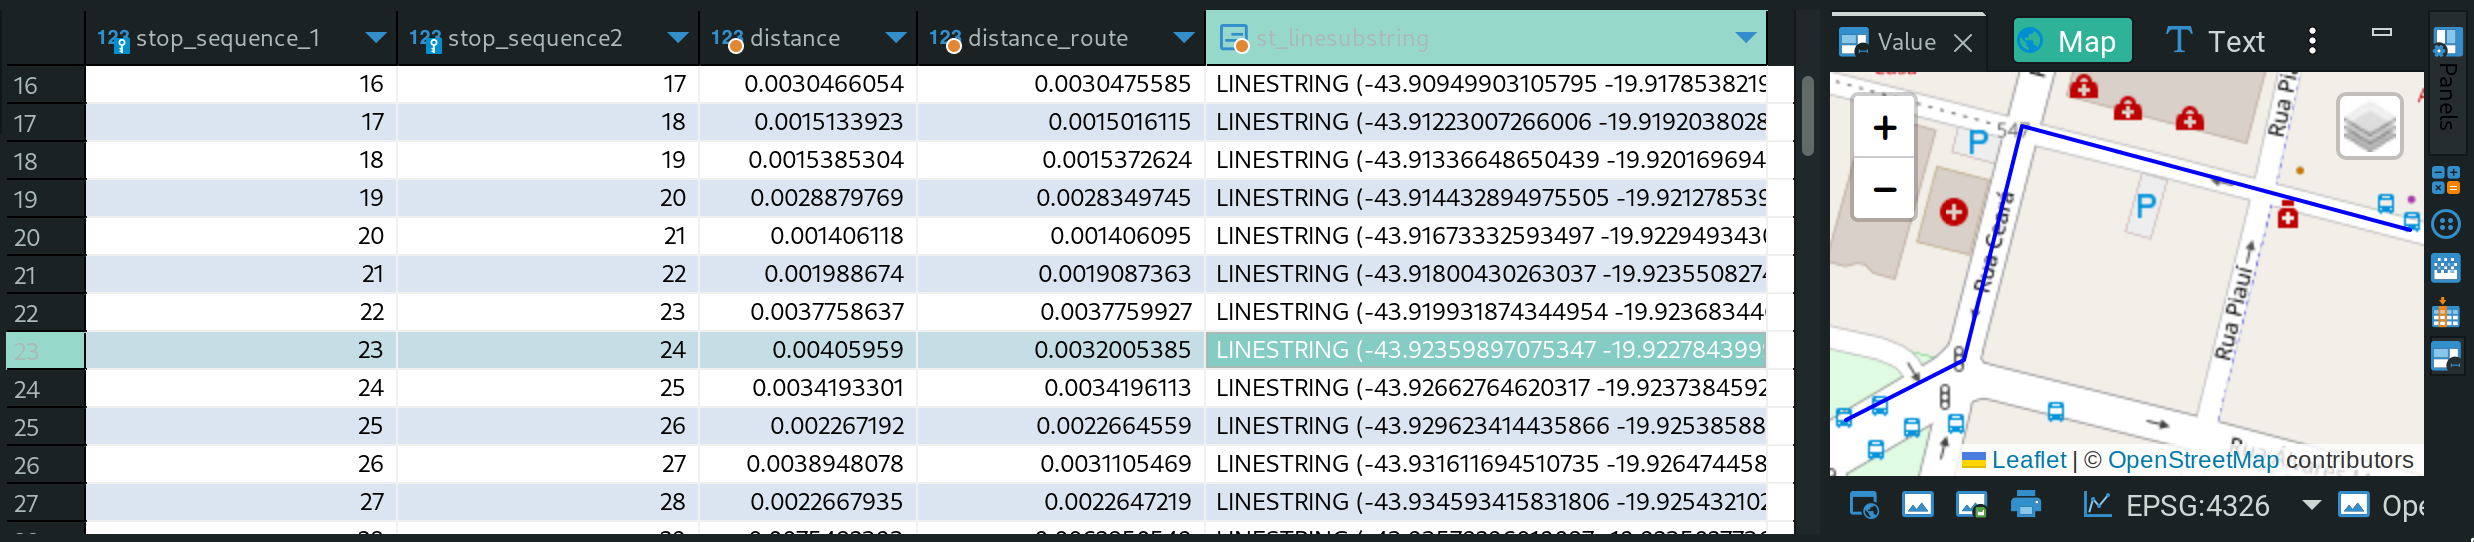
\includegraphics[width=\textwidth]{imagem/cap4/couplepoints.png}
        \source{The authors}
        \label{img:4:5}
    \end{figure}

Finally, given the building blocks, {\em Route Expected Time Generator} takes as input
routes information to calculate the average speed and route duration,
and a list of records such as Figure \ref{img:4:5}, which we iterate through leading 
to the complexity of $O(n)$. For each record, the route initial $arrival\_time$ is 
increased with the time needed to travel from a couple of bus stops at the average
speed of the route. In which {\em could} cause minor deviations to the original $departure\_time$ due to the precision 
of the calculus executed.



%TODO flag%

\subsection{Integration Driver}
The { \em Integration Driver} is the component that is composed, directly or indirectly, by the other components 
discussed in this Section to drive the execution from simple inputs as the $route\_short\_name$ and a target date
to produce a \textit{Route} instance completely filled. This component provides a default interaction not only 
between the \textit{Integration Module} components but also to the \textit{Data Providers} 
from the \textit{Data Module}.
Despite defining how the components interact, the { \em Integration Driver} depends on the abstraction
rather than the implementation, enabling the user to adapt the components to the particular scenario. Also,
it uses the default implementation with default values
for each component that is not overwritten by the user building a new instance.

    \begin{figure}[h]
        \centering
        \caption{Integration Driver Activity Diagram}
        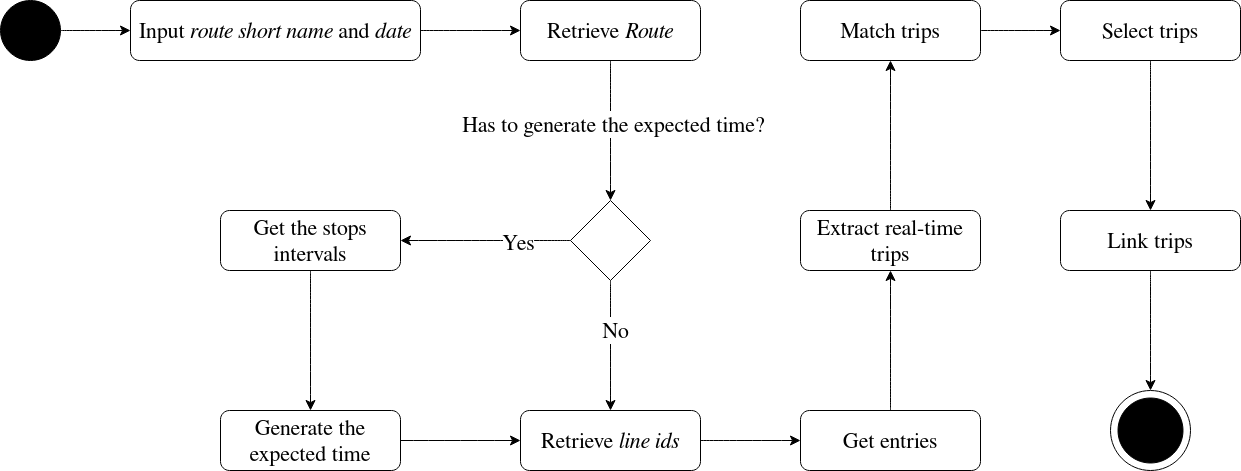
\includegraphics[width=\textwidth]{imagem/cap4/integrationDriverAD.drawio.png}
        \source{The authors}
        \label{img:4:integrationDriverAD}
    \end{figure}

Figure \ref{img:4:integrationDriverAD} shows the activity diagram of the \textit{integrate} method, which starts manipulating
the static data, then the real-time data, and finally, linking the two datasets. The first step
is to retrieve the \textit{Route} which is provided by the \textit{GTFSService} \textit{getRouteByRouteShortName}
method. Next, if the expected time at each bus stop for every \textit{Trips} of that
\textit{Route} is missing, then, before proceeding,
they are generated using the \textit{TripExpectedTimeGenerator}.
It takes the $stopsIntervals$ as input provided by the \textit{GTFSService} \textit{getStopPointsInterval} method. 
This scenario is due to the fact that the $arrival\_time$ and $departure\_time$ fields, from GTFS's $stop\_time$ 
\footnote{Available at \url{https://developers.google.com/transit/gtfs/reference#stop_timestxt}} entity is 
required just for the first and last stop of the trip.

After manipulating the static data, the next step starts by getting the $idsLines$ using the method 
\textit{getIdsLineByRouteId} from the \textit{RealTimeService}. Which is used as input to get all entries
from a day grouped by its $idVehicle$ using the method \textit{getEntriesByDtEntryAndLineIds}. In sequence, for each
vehicle, the trips are extracted in {\em parallel} using the \textit{TripExtractor}, then collected into a single
List, called $realtimeTrips$.

Finally, { \em Integration Driver} links the two datasets by matching the \textit{Route}'s \textit{Trips} 
with the real-time trips previously extracted using \textit{TripMatcher}'s \textit{match} method, that
uses a 5-minute interval, so $maxTripInitialShifting = 5$.
After matching,
it is required to select the most suitable real-time trip corresponding to a scheduled trip, which is executed by 
the \textit{TripSelector}, and the default implementation defines that a valid trip must have at least 85\% of its trajectory traveled. In other words, $tripMinPercentageTraveled = 0.85$. Then, the \textit{TripBusStopLinker}
links the bus stops with their respective entries for each scheduled trip with a real-time trip associated with,
the Driver defines a 50-meter range as the default value for $distanceThreshold$. Then, the \textit{Route} is returned.


\section{PondiônsTracker-BH}
In this Section, we present \textit{PondiônsTracker-BH}\footnote{Available at \url{https://github.com/Pongelupe/PondionsTracker-BH}} that is a \textit{PondiônsTracker}'s specialization created to
deal with Belo Horizonte's PTN particularities. So, we have implemented our own \textit{Real-Time Data collector}, and we have overwritten the method \textit{getIdsLineByRouteId} from the 
\textit{RealTimeService}.

\subsection{Real-Time Data Collector}
Belo Horizonte has a scenario similar to Rome's described in \citeonline{delays_bigdata}, in which  
different agencies provide the GTFS and real-time data. The GTFS is published
by the \textit{BHTrans}\footnote{Available at \url{https://dados.pbh.gov.br/dataset/gtfs-estatico-do-sistema-convencional}}, 
which is the local agency responsible for urban mobility planning. And 
the real-time data is provided by \textit{Transfacil}\footnote{Available at \url{https://dados.pbh.gov.br/dataset/tempo_real_onibus_-_coordenada}} which administrates the local bus services.
So, we developed our \textit{Real-Time Data Collector} in Python 3.11 to 
collect real-time data from Belo Horizonte's API.


\begin{table}[h]
\centering
\caption{Fields From The Real-Time API } 
\begin{tabular}{ |c|c|c|c| } 
\hline
Field name & Description & $real\_time\_bus$ related column \\
\hline
$EV$& Event code & - \\ 
\hline
$HR$& Timestamp & $dt\_entry$ \\ 
\hline
$LT$& WGS84 Latitude & $coord$ \\ 
\hline
$LG$& WGS84 Longitude & $coord$ \\ 
\hline
$NV$& Id vehicle & $id\_vehicle$ \\ 
\hline
$VL$& Instant speed & - \\ 
\hline
$NL$& Id line & $id\_line$ \\ 
\hline
$DG$& Vehicle's direction & - \\ 
\hline
$SV$& Trip way & - \\ 
\hline
$DT$& Distance displaced & $current\_distance\_traveled$ \\ 
\hline
\end{tabular}
\source{The authors}
\label{tab:entries-desc}
\end{table}

All entries collected were stored at $real\_time\_bus$ SQL table, but the API
has its own fields, which were translated to insert into the table. The API provides
nine fields. Table \ref{tab:entries-desc} describes each field and its translation to 
$real\_time\_bus$'s columns. 
Despite representing the $id\_line$ in the database, the $NL$ field 
is not a straightforward identifier to any GTFS entity, 
in other words, all bus entries retrieved from the API cannot be {\em directly} 
related to any trip or route. This scenario leads us to override  
\textit{RealTimeService}'s \textit{getIdsLineByRouteId} method, as further discussed
in the following Subsection.


\subsection{Belo Horizonte's \textit{RealTimeService}}
We created \textit{BHRealTimeService} to override \textit{getIdsLineByRouteId} method and use the default implementation for
the other methods, then \textit{BHRealTimeService} {\em extends} \textit{DefaultRealTimeService}. So, our implementation has to convert the
$route\_id$ using a \ac{CSV} conversion file
\footnote{Available at \url{https://dados.pbh.gov.br/dataset/tempo_real_onibus_-_coordenada/resource/150bddd0-9a2c-4731-ade9-54aa56717fb6}}
with 4 fields: $\_id$, $NumeroLinha$, $Linha$ e $Nome$. 

\begin{figure}[h]
     \centering
        \caption{Belo Horizonte's GTFS and RT data }
        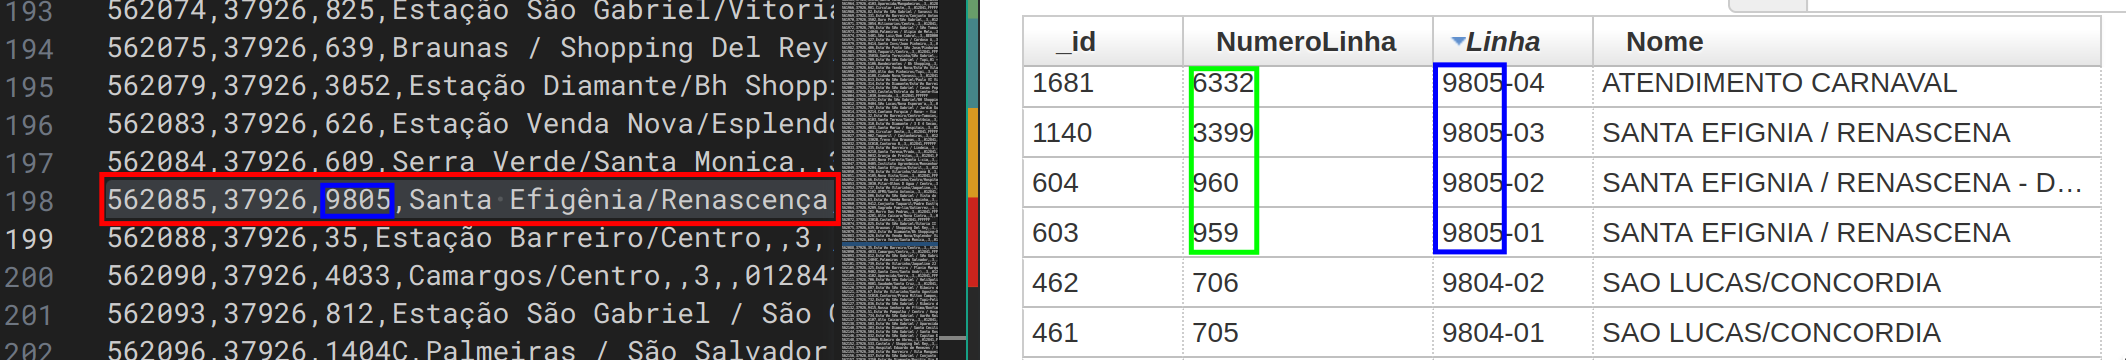
\includegraphics[width=\textwidth]{imagem/cap5/gtfsxapi.png}
        \source{The authors}
        \label{img:5:1}
\end{figure}

Figure \ref{img:5:1} shows Belo Horizontes's GTFS Routes on the left 
and the conversion table from the real-time data on the right. The first 
observation is that the column $NumeroLinha$'s domain is the $NL$, then 
$NumeroLinha = NL = id\_line$. The column $Linha$ resembles GTFS's $trip$ entity
and $routes$ relationship because it is also a \textit{one-to-many} relationship, 
in which a single bus line has multiple $Linha$ records.
For instance, the real-time API supplies an entry $e$ 
that its $NL$ is $959$, which value corresponds to an image from the domain of the 
column $NumeroLinha$ on the conversion table. Then, $959$ is going to be converted to 
$9805-01$, consequently $id\_route = 562085$.


To illustrate the \textit{one-to-many} relationship, in Figure \ref{img:5:1}
the route highlighted in red whose $route\_id$ is $562085$ has four related $NumeroLinha$ values, the group highlighted in green from the 
column $NumeroLinha$ on the conversion table. Because the group highlighted in blue
has the $route\_short\_name$ as the prefix. 
In this scenario, \textit{BHRealTimeService}'s \textit{getIdsLineByRouteId} is going
to return the group in green for $route\_id = 562085$, from the route highlighted in red.

% Nome do capítulo
\chapter{Results}
% Label para referenciar
\label{cap5}

% Diminuir espaçamento entre título e texto
\vspace{-1.9cm}

% Texto do capítulo

In this Chapter, we use Belo Horizonte as a study case to validate \textit{PondiônsTracker} using
\textit{PondiônsTracker-BH}. We used the GTFS file published on July 23${^{th}}$ 2023 and collected
data from the real-time API for eleven days straight, from 29-07-2023 to 08-08-2023.
During this period, our script was executed every minute, summarizing over 246 million entries 
representing almost 30 Gigabytes, Table \ref{tab:entries} presents the entries for each day collected.

\begin{table}[h]
\centering
\caption{Workload Overview } 
\begin{tabular}{ |c|c|c|l| } 
\hline
Date & Day-of-Week & Entries \\
\hline
29-07-23& Saturday & 22,319,765 \\ 
\hline
30-07-23& Sunday & 22,635,117 \\ 
\hline
31-07-23& Monday & 22,583,380 \\ 
\hline
01-08-23& Tuesday & 22,432,739 \\ 
\hline
02-08-23& Wednesday & 21,970,073 \\ 
\hline
03-08-23& Thursday & 22,050,579 \\ 
\hline
04-08-23& Friday & 22,402,865 \\ 
\hline
05-08-23& Saturday & 22,642,955 \\ 
\hline
06-08-23& Sunday & 22,786,254 \\ 
\hline
07-08-23& Monday & 22,109,606 \\ 
\hline
08-08-23& Tuesday & 22,405,222 \\ 
\hline
\textbf{Total}& - & \textbf{246,338,555} \\ 
\hline
\end{tabular}
\source{The authors}
\label{tab:entries}
\end{table}


We also present an analysis of the data collected, which is based on the output of 
\textit{PondiônsTracker-BH}'s \textit{IntegrationDriver} for {\em all} routes scheduled in
the GTFS during the observation period. Firstly, we compare the expected with the real scenarios of Belo Horizonte's PTN over the observed period, and then we deepen into out-of-schedule incidents, especially delays. The following analysis are divided into three groups: Weekdays, Saturday and Sunday. This happens due to the GTFS $service\_id$ field, as previously discussed in Chapter 2.


\section{Schedule Analysis}

Table \ref{tab:schedule}
shows that every observed day have $294$ \textit{Routes} planned. For weekdays are planned $22,774$ \textit{Trips},
$14,100$ for Saturdays and $9,133$ for Sundays. Table \ref{tab:schedule} shows the schedule-filled percentage of trips filled with real-time trips during the observation period. This translates to the percentage of trips planned by the trips collected and matched from the real-time API.

\begin{table}[h]
\centering
\caption{Belo Horizonte's PTN} 
\begin{tabular}{|c|c|r|r|c|}
\hline
Date & Routes    & Scheduled Trips  & Matched Trips & $\%$ \\ \hline
29-07-23 & 294 &  14,100 &     11,424   & 81.02\%\\ \hline
30-07-23 & 294 & 9,133 &  7,594  &   83.14\% \\ \hline
31-07-23 & 294 & 22,774 &  17,184  &   75.45\%  \\ \hline
01-08-23 & 294 & 22,774 &  16,948  &   74.42\%  \\ \hline
02-08-23 & 294 & 22,774 &  16,914  &   74.27\%  \\ \hline
03-08-23 & 294 & 22,774 & 16,973  &   74.53\%  \\ \hline
04-08-23 & 294 & 22,774 &  16,854  &   74.01\%  \\ \hline
05-08-23 & 294 & 14,100 &  11,372  &   80.65\%  \\ \hline
06-08-23 & 294 & 9,133 &  7,679  &   84.08\%  \\ \hline
07-08-23 & 294 & 22,774 & 16,849  &   73.98\%  \\ \hline
08-08-23 & 294 & 22,774 &  16,837  &   73.93\%  \\ \hline
\textbf{Total} & \textbf{3,234} & \textbf{205,884} &  \textbf{156,628}  &   \textbf{$76.08\%$}  \\ \hline
\end{tabular}
\source{The authors}
\label{tab:schedule}
\end{table}

\begin{figure}[h!]
     \centering
        \caption{Histograms Schedule-Filled Percentage per Routes}
        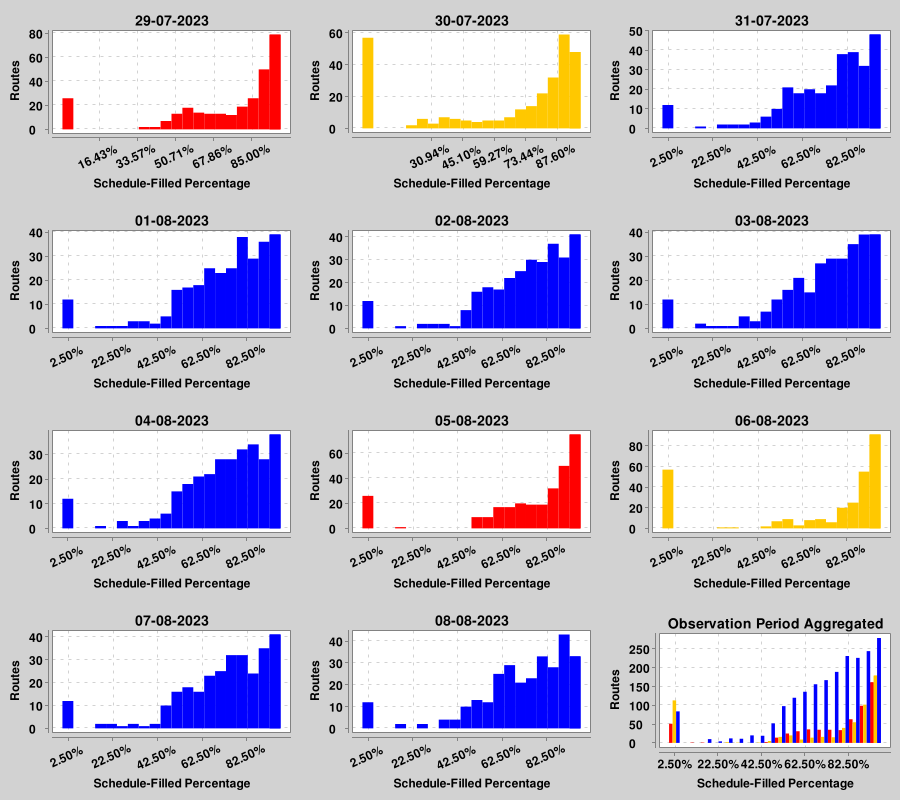
\includegraphics[width=\textwidth]{imagem/cap5/histogram_schedule-Filled.png}
        %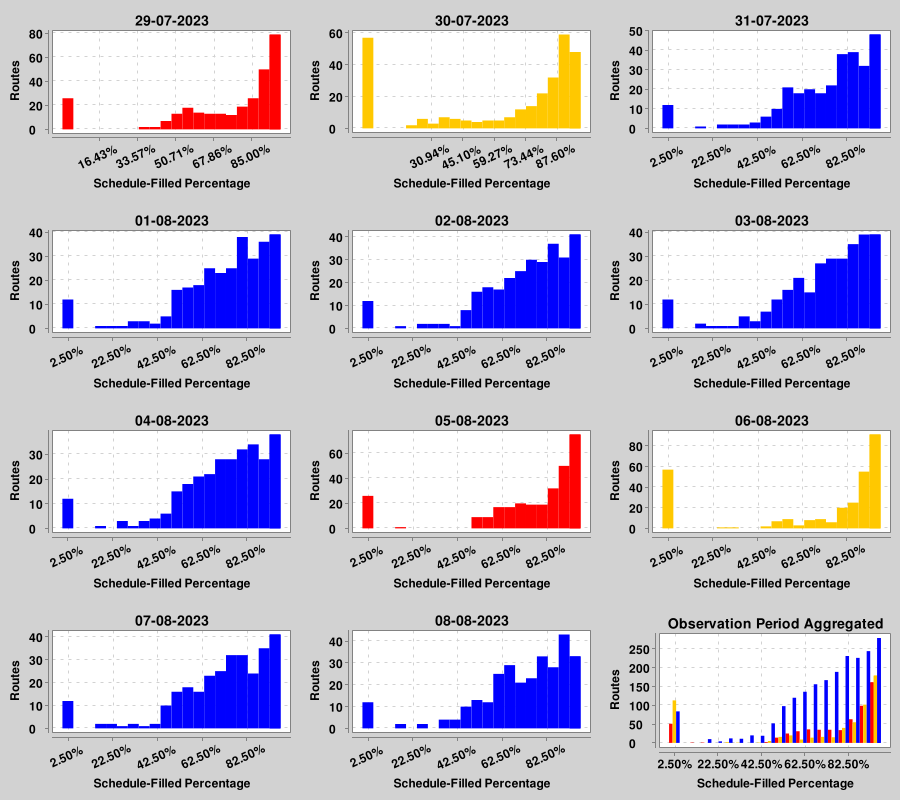
\includegraphics[scale=.3]{imagem/cap5/histogram_schedule-Filled.png}
        \source{The authors}
        \label{img:5:hist}
\end{figure}

The schedule-filled percentage values correspond to {\em all} the $3,234$ routes scheduled, and it has an average for all the period of
$76.08\%$, but this ratio is{ \em indirectly proportional} to the number of scheduled trips. 
Weekdays have the biggest number of $159,418$ trips defined and the lowest average for matched trips of
$74,37\%$, comprised by 31-07, 01-08, 02-08, 03-08, 04-08, 07-08 and 08-08.
Saturday's average is $80.84\%$ with $28,200$ scheduled trips, comprised of days 29-07 and 05-08.
Finally, Sunday's average is $83.61\%$ with $18,266$ scheduled trips comprised of days 30-07 and 06-08.

Figure \ref{img:5:hist} shows the histograms of the schedule-filled percentage distributed throughout each day, and
the last histogram presents the aggregated distribution for the observation period. The red, yellow, and blue bars represent Saturday, Sunday, and Weekdays. All histograms present that the schedule is not uniformly distributed,
and despite the averages shown in Table \ref{tab:schedule}, for each day, the most considerable individual 
frequencies are associated with the schedule-filled percentage of at least $82.50\%$, as shown in the aggregated histogram. 

All histograms show the existence of considerable sets of routes whose schedule-filled percentage is {\em at most} $42.50$\%, and, especially, routes with near 0 routes reported. These sets are 
likely caused by the unpredictable and randomness of the network, leading to unwanted and unfinished trips, as discussed in the previous Chapter. Which decreases the averages and points to a high standard deviation, representing that the schedule is not uniformly distributed. Then, plenty of routes are completed ($100\%$) or at least near $82.50\%$, despite some associated with lower percentages.


Regarding the real-time API, there are $4,095$ collected trips from $63$ different routes which were not defined at Belo 
Horizonte's GTFS. In other words, the API provided $4,095$ trips with a valid $NV$ unscheduled 
trips. Table \ref{tab:unscheduledTrips} shows the top 5 routes with the most unscheduled trips. 
For instance, the route $82$ has a high schedule-filled rate  with real-time trips despite having the most
unscheduled trips. On Sundays, the GTFS does not schedule any trip for route $82$,
but the API provided 
entries regarding this route twice during the period observed.
The first time with $147,897$ entries leading to $505$ trips collected 
and the second time with $149,422$ entries leading to $551$ trips collected , then once added gets to the $1,056$ shown in Table \ref{tab:unscheduledTrips}.

\begin{table}[h]
\centering
\caption{Top 5 Routes With The Most Unscheduled Trips} 
\begin{tabular}{|l|c|}
\hline
Route & Unscheduled Trips  \\ \hline
\textit{82 - Estação São Gabriel / Savassi Via Hospitais} & 1,056 \\ \hline
\textit{61 - Estação Venda Nova/Centro-Direta} & 791 \\ \hline
\textit{52 - Estação Pampulha / Avenida Antonio Carlos} & 612 \\ \hline
\textit{50 - Estação Pampulha / Centro - Direta} & 309 \\ \hline
\textit{85 - Estação São Gabriel / Centro Via Floresta} & 257 \\ \hline
\end{tabular}
\source{The authors}
\label{tab:unscheduledTrips}
\end{table}



\section{Delay Analysis}
To analyze the delays in the PTN, firstly, we take a look at the delays on a global scale of the network, and for the context of this section, to be {\em on-time} denotes that the expected time is equal to the real-time
within a maximum fifty-nine-seconds span, so a {\em delay} is a time after the expected and a {\em ahead-of-schedule}
is a time before the expected, with equal or greater than one minute.
In this context, Table \ref{tab:delay1} presents data over the matched trips aggregated by the day of the week, 
in which the trips entirely out of schedule represent the most extensive set of trips. The definition of this group is that every trip 
does not have a single entry on time. In other words, for these trips, the buses were either delayed
or ahead of schedule for all expected times at every bus stop. 



\begin{table}[h]
\centering
\caption{Delays detailed in whole PTN scale } 
\begin{tabular}{|l|r|r|r|}
\hline
\multicolumn{1}{|c|}{} & Weekday    & Saturday    & Sunday  \\ \hline
Total trips  matched & 118,559 &  22,796  & 15,273\\ \hline
Trips entirely out of schedule & 60,244  & 10,899 & 7,148\\ \hline
Trips with departure or arrival on time & 39,403 & 8,731 &    5,988\\ \hline
Trips with departure and arrival on time & 324 & 95 & 56 \\ \hline
Trips entirely on time & 1 & 2 &  1\\ \hline
\end{tabular}
\source{The authors}
\label{tab:delay1}
\end{table}

Furthermore, Table's \ref{tab:delay1} second and third
most extensive sets are related to trips that are on-time at the beginning and the end of the trip. The
third group represents if the trip is on time on both ends, and it is contained by the second group, which requires
at least one end on time. The second group also contains the last group, a particular case of the bus being on time for {\em all} bus stops in the trip, which occurred only four times during the observation period for the same route, coincidentally.
The route is \textit{331 - Estação Barreiro/Conjunto Antonio Teixeira Dias Via Upa}, which has 32 bus stops, representing a length of 8,948.92 meters, almost 9 kilometers, and the four expected and real date-times are listed as follows:
\begin{enumerate}
    \item Expected departure and arrival: Jul. 29 15:30:00 - 15:56:27 \\ Real departure and arrival: Jul. 29 15:30:03 - 15:57:03;
    \item Expected departure and arrival: Jul. 30 08:20:00 - 08:46:27 \\ Real departure and arrival: Jul. 30 08:20:31 - 08:46:15;
    \item Expected departure and arrival: Aug. 04 05:40:00 - 06:06:27 \\ Real departure and arrival: Aug. 04 05:40:30 - 06:06:00;
    \item Expected departure and arrival: Aug. 05 17:10:00 - 17:36:27 \\ Real departure and arrival: Aug. 05 17:10:45 - 17:36:49.
\end{enumerate}

\begin{figure}[h!]
     \centering
        \caption{$DELAY$s Distribution: Bus Stop and Trip}
        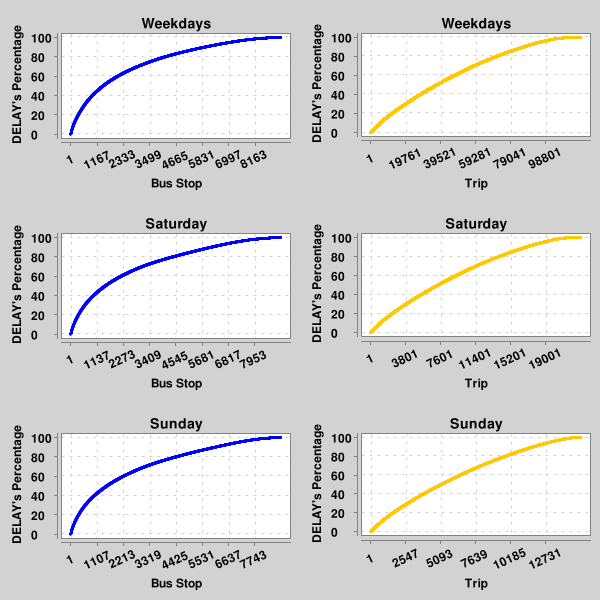
\includegraphics[scale=.45]{imagem/cap5/trips_delays_per_bus_stops.png}
       % 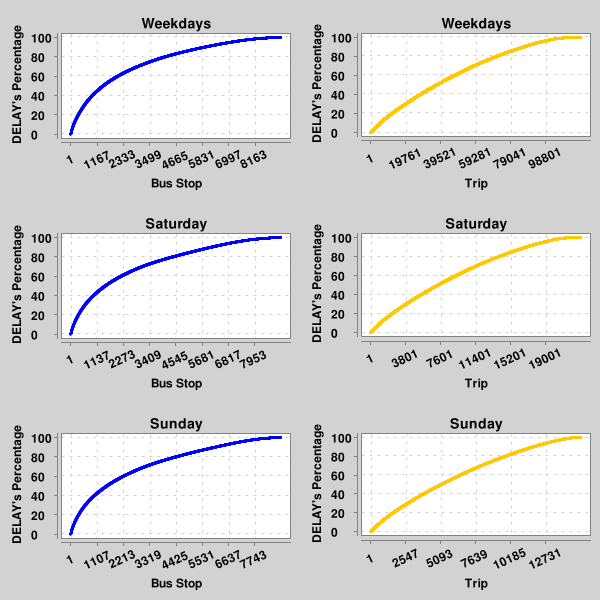
\includegraphics[width=\textwidth]{imagem/cap5/trips_delays_per_bus_stops.png}
        \source{The authors}
        \label{img:5:DelayDistribution}
\end{figure}

Until this point, our analysis has not taken into account the impact of each distinct status in the PTN, and for weekdays, the statuses are divided as:
\begin{enumerate*}
    \item DELAY representing $89.8\%$;
    \item AHEAD\_OF\_SCHEDULE representing $6.9\%$;
    \item ON\_TIME representing $3.3\%$.
\end{enumerate*}
The predominance of $DELAYED$ in the PTN does not imply that the network is not working 
nor completely stopped because the $DELAYED$s are {\em log-normal} distributed between the bus stops and trips, as shown in Figure \ref{img:5:DelayDistribution}.
So, this leads to the scenario where few bus stops and trips cause more delays. 
For instance, for all delays reported for weekdays, 200 trips represent $14.05\%$, and 200 bus stops $73.75\%$. This distribution also occurs on Saturdays and Sundays, as shown in Figure \ref{img:5:DelayDistribution}.



The distribution indicates a small set of bus stops is responsible for most delays, but it does not imply any spatial relationships between this set. Figure \ref{img:5:mostDelayedStops} shows $2,115$ out of $9,309$ most delayed bus stops, representing around $60\%$ of the total delay and only $22.72\%$ of the bus stops. It is observable that some main avenues
and pathways are contemplated, such as the following:
\begin{enumerate*}
    \item \textit{Avenida Dom Pedro II};
    \item \textit{Rua Padre Eustáquio};
    \item \textit{Avenida Amazonas}.
\end{enumerate*}

\begin{figure}[h]
\centering
\begin{minipage}[t]{.5\textwidth}
  \centering
  \caption{300 Most Delayed Stops}
  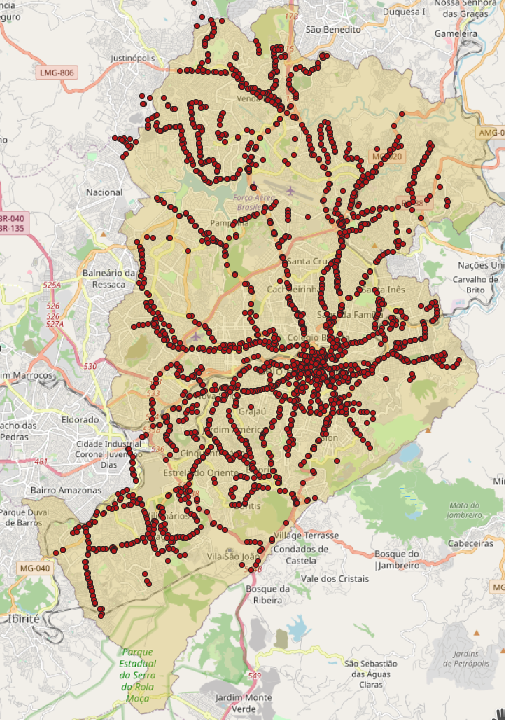
\includegraphics[width=.90\linewidth]{imagem/cap5/mostDelayedStops.png}
  \source{The authors}
  \label{img:5:mostDelayedStops}
\end{minipage}%
\begin{minipage}[t]{.5\textwidth}
  \centering
  \caption{Fragment of the 50 Most \\Delayed Stops }
  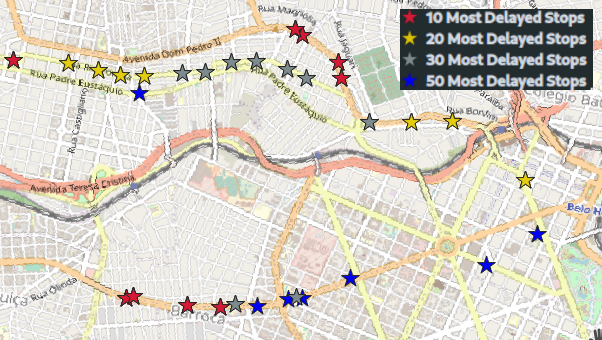
\includegraphics[width=\linewidth]{imagem/cap5/10-50MostDelayedStops.png}
  \source{The authors}
  \label{fig:50mostDelayedStops}
\end{minipage}
\end{figure}

These three pathways are represented in Figure \ref{fig:50mostDelayedStops}, which shows a 
fragment of Belo Horizonte's PTN and indicates the 50 most delayed stops divided into groups
regarding the number of delays. So, the stops in red accumulate the most delays, and
the group in blue gathers the fewest for this figure, yet these stops represent $4.58$\% of the network.
Also, Figure \ref{fig:50mostDelayedStops} reveals the spatial relationships between these stops
because they are on the same pathway. For instance, the \textit{Avenida Amazonas}, the avenue located in the lower part of the figure, is one of the most critical avenues in the PTN, containing dozens of stops throughout its 8.97 kilometers, \textit{Avenida Amazonas} has 10 out of the 50 most delayed
stops. As follows, we list the 5 most delayed stops for weekdays during the observation period:

\begin{enumerate}
    \item $\#14793268$ - \textit{Avenida Dom Pedro II 1520} with $7,309$ delays reported at;
    \item $\#14791617$ - \textit{Avenida Amazonas 7309} with $7,009$ delays reported at;
    \item $\#14790997$ - \textit{Avenida Dom Pedro II 1980} with $6,692$ delays reported at;
    \item $\#14784438$ - \textit{Avenida Sinfronio Brochado 773} with $6,528$ delays reported at;
    \item $\#14788981$ - \textit{Avenida Amazonas 3410} with $6,272$ delays reported at.
\end{enumerate}


\begin{figure}[b]
     \centering
        \caption{Minutes out of schedule of bus stops $\#14788408$ distributed throughout the day}
        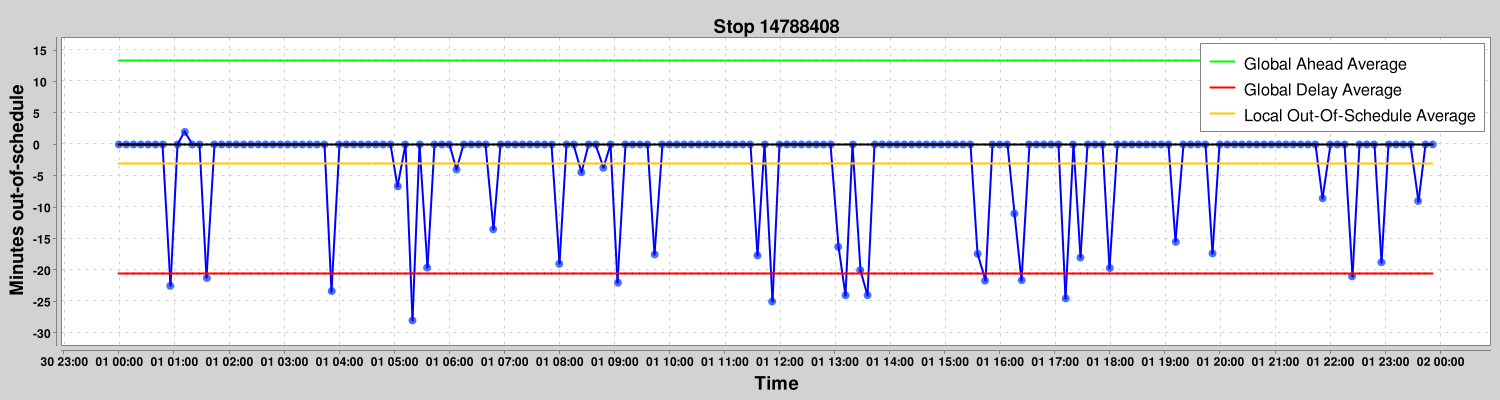
\includegraphics[width=\textwidth]{imagem/cap5/stops1.png}
        \source{The authors}
        \label{img:5:stops2}
\end{figure}

Despite pointing to the spatial relationship between the stops, Figures \ref{img:5:mostDelayedStops} and \ref{fig:50mostDelayedStops} fail to provide a temporal association. This is relevant because
the PTN is dynamic, not a framed snapshot, so bus stops may be physically close and unaffected by each other, and for instance,
a couple of bus stops on opposite sides of the same avenue.
Also, the delays occur sparsely during the day, and not all delays 
are caused by the same causes.
For illustration, a delay caused by a flat tire is different from one caused by a traffic jam, and 
a delay reported in the morning is unlikely to affect another from hours later, and so on.

Figure \ref{img:5:stops2} represents the stop whose $stop\_id$ is $\#14788408$, it is located at \textit{Rua Indiana 135}, and is a bus stop that is not on a busy pathway nor has significant delays to the PTN. But this stop exemplifies the behavior of the delays
over the hours of the day. The $y-axis$ represents the average minutes of all out-of-schedule statuses at that stop grouped by 
8-minute intervals, in which negative values represent delays and positive ahead-of-schedule, and the $x-axis$ is the time of the day. Also, the following three constants are displayed:
\begin{enumerate}
    \item \textit{Global Ahead Average}: $13.42$ minutes that represents the average of ahead-of-schedule in the PTN in green;
    \item \textit{Global Delay Average}: $20.49$ minutes that represents the average of delay in the PTN in red;
    \item \textit{Local Out-Of-Schedule Average}: The average number of minutes out-of-schedule for that given bus stop in yellow.
\end{enumerate}

\begin{figure}[b!]
     \centering
        \caption{Minutes out of schedule of a couple of bus stops distributed throughout the day}
        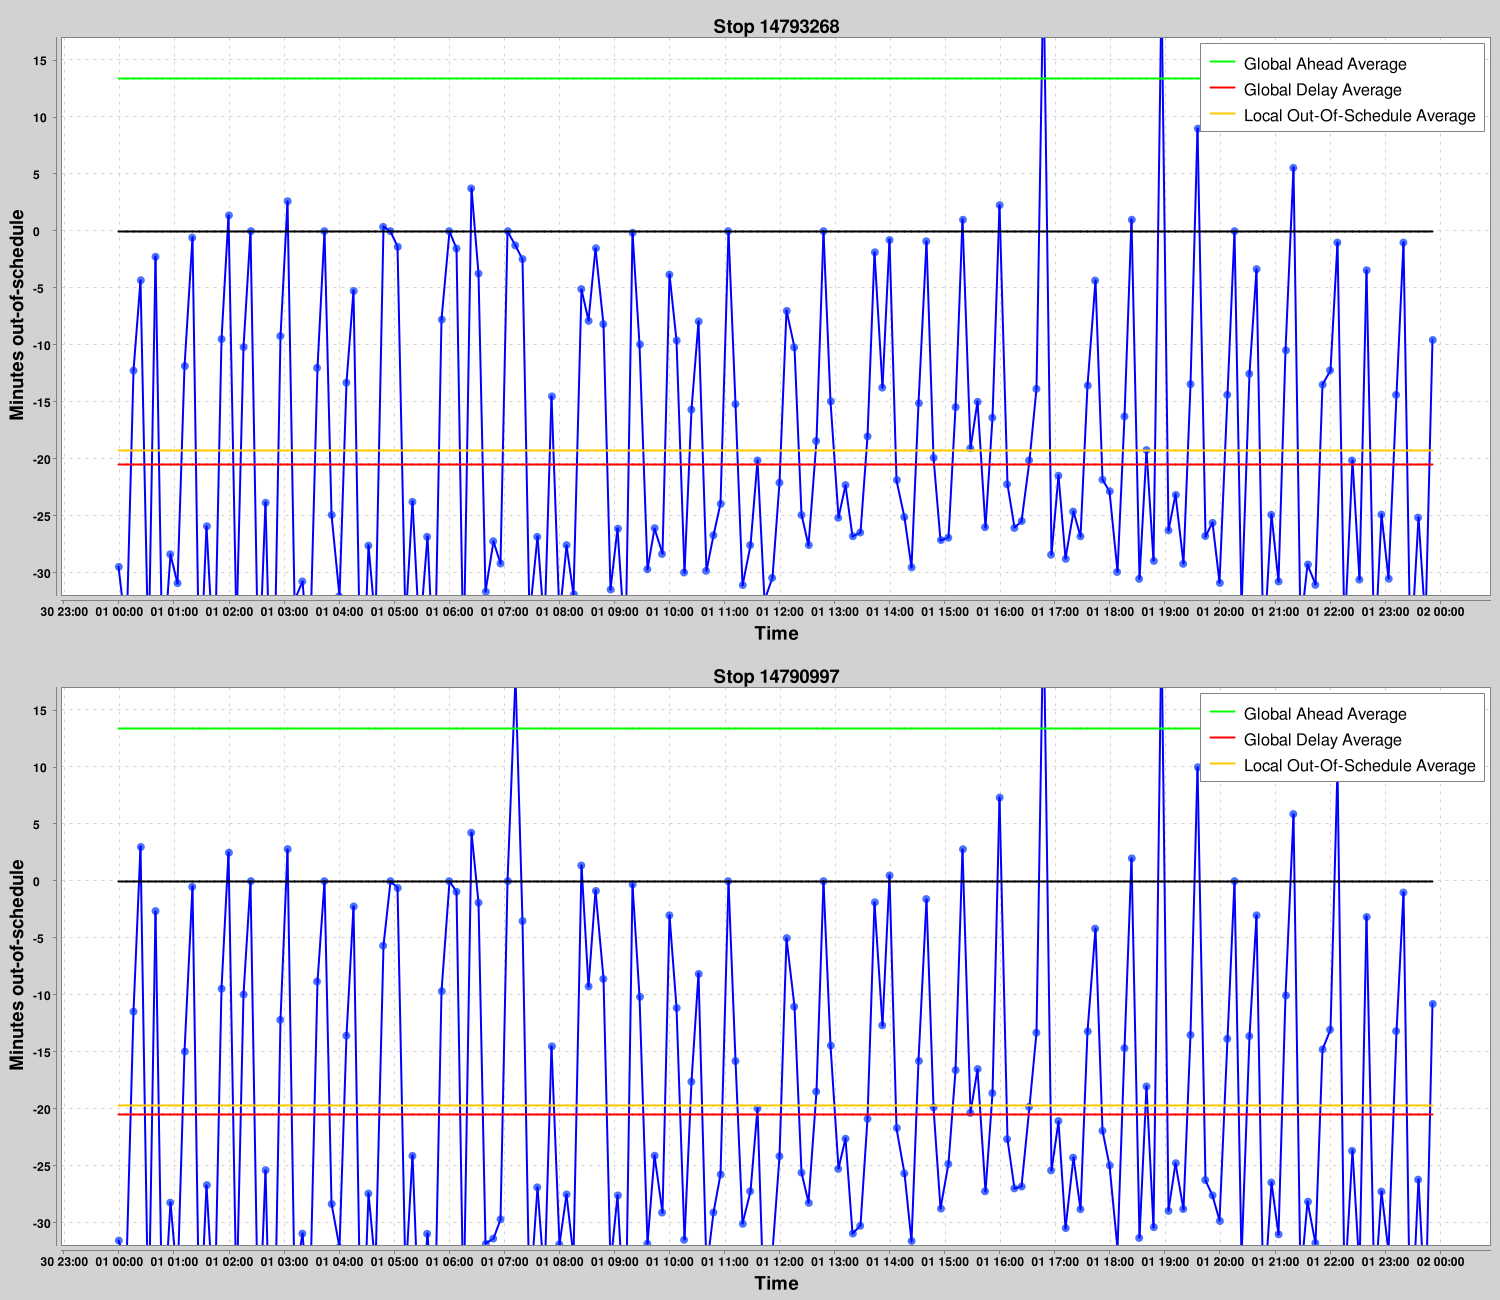
\includegraphics[width=\textwidth]{imagem/cap5/stops2.png}
        \source{The authors}
        \label{img:5:stops}
\end{figure}

For instance, using stop $\#14788408$, each blue dot in Figure \ref{img:5:stops2} denotes the average
minutes out-of-schedule for this stop in an instant in time. So, around 1:15 A.M., all the buses heading to this stop had an average
of 2 minutes ahead of schedule, and around 21:50 A.M., all the buses heading to this stop had an average of 9 minutes delayed.
Since the green and the red constants are global averages, they are unreliable for analyzing the delays due to the {\em log-normal}
distribution, but the yellow gives a more reliable insight to create a time-window interval, so for 
this stop, on average, the buses are delayed 3 minutes.


The stops $\#14793268$ and $\#14790997$ are the first and third most delayed in the PTN, respectively.
These stops are 462 meters from each other on the same avenue, \textit{Avenida Pedro II}, and share 2,590 common trips, so they are spatially related. Furthermore, they also have a temporal relationship, and 
Figure \ref{img:5:stops} works similarly to Figure \ref{img:5:stops2} and shows these stops on weekdays. Observing Figure \ref{img:5:stops}, the similarities of
delay distribution in these stops demonstrate the temporal relationship because 
both stops have similar frequencies of all statuses simultaneously: on time, ahead of schedule, and delayed. For instance, the early morning period from 4:00 A.M. to 7 A.M. is
practically equal with periods of intense delays, while the afternoon period starting at 5:00 P.M. reveals for both stops trips ahead of schedule. Also, these stops have a close \textit{Local Out-Of-Schedule Average}, which is $19.29$ minutes for $\#14793268$ and $19.68$ for minutes $\#14790997$, both are delays.



\section{Comparison Between Generated and Real Data}
The analysis shown in the two previous sections was only possible because Belo Horizonte's GTFS defines the expected time for all
bus stops on every trip. Belo Horizonte's GTFS provides this data despite not being required fields. 
As discussed in the previous Chapter, the \textit{Trip Expected Time Generator} generates the expected times when missing. In this section, we executed this component with Belo Horizonte's data and compared the expected times generated
with those defined at the GTFS. Table \ref{tab:delay2} displays the same data presented in Table \ref{tab:delay1}
but increasing it with the generated expected times.

\begin{table}[h]
\centering
\caption{Delays detailed in whole PTN scale with generated expected times}
\begin{tabular}{|c|c|c|r|r|}
\hline
\multicolumn{3}{|c|}{} &   GTFS  &  Generated  \\
\hline
 \multirow{5}{*}{\textbf{Weekday}} & \multicolumn{2}{|c|}{\textbf{Total trips matched}} &118,559 &  118,559 \\\cline{2-5}
 & \multicolumn{2}{|c|}{\textbf{Trips entirely out of schedule}} &60,244  & 57,843 \\\cline{2-5}
 & \multicolumn{2}{|c|}{\textbf{Trips with departure or arrival on time}} &39,403 & 39,526  \\\cline{2-5}
 & \multicolumn{2}{|c|}{\textbf{Trips with departure and arrival on time}} &324 & 393\\\cline{2-5}
 & \multicolumn{2}{|c|}{\textbf{Trips entirely on time}} &1&0 \\
\hline
 \multirow{5}{*}{\textbf{Saturday}} & \multicolumn{2}{|c|}{\textbf{Total trips matched}} &22,796 &  22,796\\\cline{2-5}
 & \multicolumn{2}{|c|}{\textbf{Trips entirely out of schedule}} & 10,899  & 10,497 \\\cline{2-5}
 & \multicolumn{2}{|c|}{\textbf{Trips with departure or arrival on time}} &8,731 & 8,723  \\\cline{2-5}
 & \multicolumn{2}{|c|}{\textbf{Trips with departure and arrival on time}} &95 & 130 \\\cline{2-5}
 & \multicolumn{2}{|c|}{\textbf{Trips entirely on time}} &2&0 \\
\hline
 \multirow{5}{*}{\textbf{Sunday}} & \multicolumn{2}{|c|}{\textbf{Total trips matched}} &15,273 &  15,273\\\cline{2-5}
 & \multicolumn{2}{|c|}{\textbf{Trips entirely out of schedule}} & 7,148  & 6,733 \\\cline{2-5}
 & \multicolumn{2}{|c|}{\textbf{Trips with departure or arrival on time}} &5,988 & 6,022  \\\cline{2-5}
 & \multicolumn{2}{|c|}{\textbf{Trips with departure and arrival on time}} &56 & 73 \\\cline{2-5}
 & \multicolumn{2}{|c|}{\textbf{Trips entirely on time}} &1&0 \\
\hline
\end{tabular}
\source{The authors}
\label{tab:delay2}
\end{table}

Table \ref{tab:delay2} shows that our generated data has some similarities and differences to the provided data and
using the generated data, Weekdays, Saturdays, and Sundays have fewer trips entirely out of schedule, $3.99$\%, $3.69$\%, and
$5.81$\%, respectively. 
On the one hand, this decrease points to a redistribution of the status $ON\_TIME$ throughout the network. %because the gross number of this status has decreased, as Figure \ref{img:5:pie} shows
On the other hand, this redistribution affected the four trips entirely on time, which are missing. 
Another point is that for all cases, except one, the generated schedule has
increased the number of trips with departure and/or arrival on time, and this occurs due to the minor alterations to the 
$departure\_time$ field caused by the \textit{DefaultTripExpectedTimeGenerator}, which were used. 
Saturday's trips with departure or arrival on time is the scenario that the generated data was outperformed by $0.09$\%,
virtually, they performed equally. 

Furthermore, Table \ref{tab:delaydistribution} presents statuses throughout the bus stops for the GTFS and the expected times
generated. For both scenarios, the $DELAYED$ status is predominant in the network, followed by the $AHEAD\_OF\_SCHEDULE$ and
$ON\_TIME$, respectively. Also, Table \ref{tab:delaydistribution} shows an expressively increase in $AHEAD\_OF\_SCHEDULE$
, and an expressively decrease for $DELAYED$, and a minor decrease for $ON\_TIME$ when using the generated data. 
Despite the $DELAYED$ status having the most occurrences, it does not denote that the PTN is completely stopped or delayed due to the
{\em log-normal} distribution of this status, as discussed in the previous Section.

\begin{table}[h!]
\centering
\caption{Statuses Distribution for Bus Stops}
\begin{tabular}{|c|c|c|r|r|}
\hline
\multicolumn{3}{|c|}{} &   GTFS  &  Generated  \\
\hline
 \multirow{3}{*}{Weekday} & \multicolumn{2}{|c|}{$ON\_TIME$} & $3.3\%$ & $3.2\%$ \\\cline{2-5}
 & \multicolumn{2}{|c|}{$AHEAD\_OF\_SCHEDULE$} & $6.9\%$ & $17.8\%$ \\\cline{2-5}
 & \multicolumn{2}{|c|}{$DELAYED$} &$89.8\%$ & $79.0\%$  \\
\hline
 \multirow{3}{*}{Saturday} & \multicolumn{2}{|c|}{$ON\_TIME$} & $3.9\%$ & $3.5\%$ \\\cline{2-5}
 & \multicolumn{2}{|c|}{$AHEAD\_OF\_SCHEDULE$} & $6.5\%$ & $18.4\%$ \\\cline{2-5}
 & \multicolumn{2}{|c|}{$DELAYED$} &$89.6\%$ & $78.1\%$  \\
\hline
 \multirow{3}{*}{Sunday} & \multicolumn{2}{|c|}{$ON\_TIME$} & $4.4\%$ & $3.9\%$ \\\cline{2-5}
 & \multicolumn{2}{|c|}{$AHEAD\_OF\_SCHEDULE$} & $5.4\%$ & $18.5\%$ \\\cline{2-5}
 & \multicolumn{2}{|c|}{$DELAYED$} &$90.2\%$ & $77.6\%$  \\
\hline
\end{tabular}
\source{The authors}
\label{tab:delaydistribution}
\end{table}


Finally, Figure \ref{img:5:stops_generated} presents the same couple of stops from Figure \ref{img:5:stops} but using the
generated expected times. With the generated data, the \textit{Global Ahead Average} and the \textit{Global Delay Average}
are $38.57$ and $24.75$ minutes, respectively. This denotes that the interval of out-of-schedule is wider using the generated data. Still, on the other side, the \textit{Local Out-Of-Schedule Average} show smaller delays for the stops $\#14793268$ and $\#14790997$, $15.54$ and $14.68$ minutes respectively. This data points out that despite increasing the global averages, our 
approach decreased the average delay in two of the most delayed stops from the PTN by $3.75$ and $5$ minutes, respectively.

\begin{figure}[h]
     \centering
        \caption{Minutes out of schedule of a couple of bus stops distributed throughout the day using generated data}
        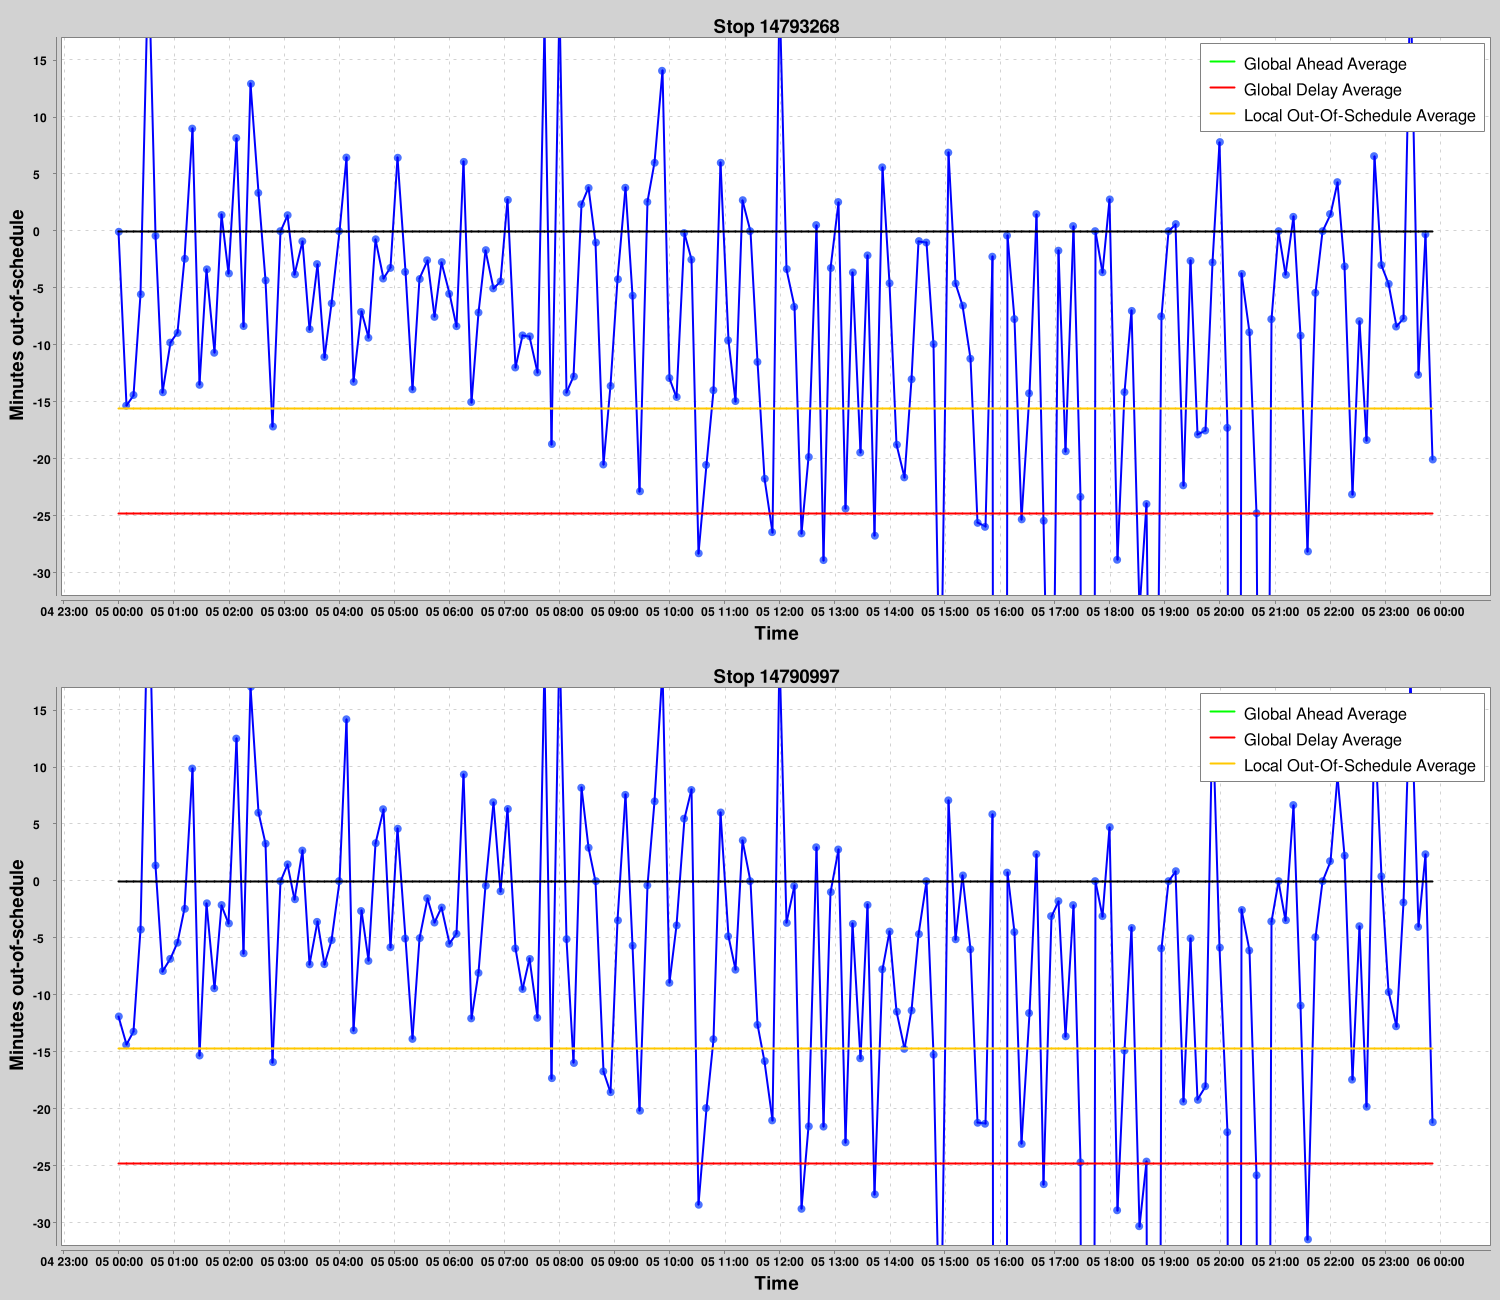
\includegraphics[width=\textwidth]{imagem/cap5/stops2_generated.png}
        \source{The authors}
        \label{img:5:stops_generated}
\end{figure}

\section{Limitations}
We acknowledge some limitations, mainly due to the desynchronization
between the datasets. For instance, the {\em Real-Time Data Collector} is the most fragile component due
to the third-party real-time traffic API interface, which creates minor issues,
such as providing some unwanted trips. And some significant problems, such as 
the impossibility of linking an entry to a trip. Also, the crucial point is that the size and quality of 
the real-time data heavily depend on the API refresh timeout, in which smaller
timeouts translate to more bus positioning, which improves the accuracy of generating
artificial entries.

We acknowledge the lack of methods to make a comparison, we discussed about all the others similar scenarios found in literature in Chapter 3.
Also, \textit{PondiônsTracker} fails to capture unexpected events that affect the traffic such as concerts because these events {\em may} not be represented by the GTFS. 
Thus, two routes are scheduled in the GTFS, but they did not have any entry reported by the real-time API, which are 
the two following routes:
\begin{enumerate*}
    \item \textit{720 - Circular Saúde MG20} missed $175$ trips;
    \item \textit{912 - Conjunto Taquaril/Praça Che Guevara} missed $210$ trips.
\end{enumerate*}


% Nome do capítulo
\chapter{Concluding Remarks}
% Label para referenciar
\label{cap5}

% Diminuir espaçamento entre título e texto
\vspace{-1.9cm}

In this master dissertation, we present \textit{PondiônsTracker}, a framework used to collect and
integrate GTFS and real-time data. Then, we validate our framework by specializing it to work with Belo Horizonte, \textit{PondiônsTracker-BH}. We collected data from the real-time API for eleven days straight, summarizing over 253 million entries in 2023 and combining it with Belo Horizonte's GTFS data to analyze 
its PTN. 

Our analysis compares the expected schedule with the actual schedule, which uncovers some gaps between
the schedule defined at the GTFS and the data collected at Belo Horizonte. First, there are a couple of routes, representing 385 trips the API has not reported at least one entry, and others 200 that have no matched trip, despite having reported entries. 
This scenario shows a lack of information from the real-time data provider. Also, this analysis points out
to the fact that the GTFS data provider under-scheduled trips, which were returned by the API.

Also, we shed light on some delay analysis using the expected times defined at the GTFS and the expected times
generated by the \textit{Trip Expected Time Generator}. The performance of the generated dataset shows that the
component is a viable option when the stop times are not defined. Belo Horizonte's data 
demonstrates that only four out of over 150 million trips were entirely on time compared to the schedule, and there are
many trips entirely out of schedule. This denotes how complex the PTN of a major city can get and points to the open
questions about delays currently being researched in the literature. 

Regarding delays in Belo Horizonte's PTN, we show that delays are the most predominant status concerning the schedule. 
They follow a {log-normal} distribution throughout the bus stops and might be both spatial and temporal related.
This scenario supplies substrate to guide the local programs and initiatives to address mobility issues because it
is the right of the citizens to transit around their city, and it directly affects thousands of people in a daily routine. 
Also, a concise PTN plays a significant role in approaching climate change questions because it could replace 
several individual vehicles with a few collective ones, for instance.

The analysis performed over Belo Horizonte was only possible because \textit{PondiônsTracker} enabled
the link between the two datasets because of the nonexistence of GTFS-RT. 
Developing, validating, and, mainly, sharing \textit{PondiônsTracker}
to as many cities as possible to analyze their data when the GTFS-RT is unavailable is our main
contribution in this master thesis. This is translated to \textit{PondiônsTracker} architecture, which
takes loose coupling as principal, and the \textit{DataProviders} and \textit{IntegrationModule}'s all components are available as Maven dependencies. 
Furthermore, the \textit{IntegrationModule} provides many components that are planned to be used as 
building blocks, so for each particular city, the different blocks can be adapted and combined. 
The \textit{IntegrationDriver} executes a default sequence of steps to unify the two datasets into a 
single SQL schema, which schema could have been created and populated by the shell script provided, $init.sh$.

As future work, we intend to explore Belo Horizonte's PTN further, then collect wider time intervals
and apply deep learning for graph techniques. 
This toolkit can explore the impact of different bus stops on each other, even if
they are apparently unrelated, such as two stops from different neighborhoods.
Thus, graphs algorithms that explore shortest path may show delay patterns and methods to mitigate them.
Also, \textit{PondiônsTracker} can be incorporated to geovisualization tools such Layerbase \cite{layerbase}. 
In addition, \textit{PondiônsTracker-BH} output, the base of all analysis, can be used as input for a deep graph network. For instance, state-of-the-art 
techniques such as Flock of Starlings can be exploited.

Also, in future work, we intend to reproduce the results obtained in Belo Horizonte in other cities, not
restrained to Brazil. It is an opportunity to improve human mobility in smart cities without the GTFS-RT but with multiple providers, as described in \citeonline{delays_bigdata}. Finally, in future work, further exploring the PTN delays combining temporal and spatial dimensions because vehicles in 
the same pathway will get stuck{ \em together} in a traffic jam, and a slow pace of traffic during rush hour follows the same principle, for instance.


% PÓS-TEXTUAIS %%
% Bibliografia no arquivo 'Dissertacao.bib'
% Alterar o título das referências para somente 'Referências'
%\renewcommand{\bibname}{References}
\renewcommand{\refname}{References}
\bibliographystyle{abnt-alf}
\bibliography{Dissertacao.bib}

% Para forçar que os apêndices e anexos comecem no anverso
%\setboolean{@openright}{true}

\end{document}
